% Important: The shell-escape flag is required for the Minted package.
% Please compile this document with 'pdflatex -shell-escape main.tex'.
% If you are using another IDE, you may be able to specify this in the
% options or to provide an option like '% !TEX option = -shell-escape'
% in this file, depending on your builder. See the README.md for more.

% Don't put any content in here.
% Don't even include content files by using \input or \inlcude.
% Put your content into components/text.tex or include it there using \input.
% You probably want to modify the following files:
%   components/info.tex             contains the author, title etc.
%   components/settings.tex         contains the packages and settings.
%   components/commands.tex         contains helpful custom commands.
%   components/glossary.tex         contains an explanation of the used terms.
%   components/acknowledgements.tex contains the acknowledgements.
%   components/quote.tex            contains a quote.
%   components/abstract.tex         contains the abstract of the document.
%   components/text.tex             includes the actual content of the document.
%   components/outline.tex          contains the outline.
%   components/preface.tex          contains the preface.
%   chapters/                       contains the main text.
%   bibliography/literature.bib     contains the BibTeX entries.
%   images/                         contains all your content-related images.
%
% You probably don't need to change anything in the following files:
%   components/cover.tex            formats the front cover of the document.
%   components/titlepage.tex        formats the title page of the document.
%   components/disclaimer.tex       formats the disclaimer page.
%   styles/                         contains style elements (e.g. logos).
%   main.tex                        contains the top-level code structure.
%   README.md                       contains information about this template.

\documentclass[11pt,
              a4paper,
              index=totoc,
              headsepline,
              footsepline,
              BCOR=12mm,
              DIV=13]{scrbook}

% KOMA scrbook options:
%  index=totoc: include an entry for the index in the table of contents.
%  headsepline: use horizontal line under heading.
%  footsepline: use horizontal line above footer.
%  BCOR: binding correction (e.g.: BCOR=12mm)
%  DIV: Number of sheet sections (used for layout) (e.g.: DIV=13)


%  This code base is currently hosted at: 
%  https://github.com/waltsims/TUM_Thesis_Template_CSE
             
% !TEX root = ../main.tex
% Set here the title, authors and other stuff to be used for the cover
% This file is used by MAIN.TEX

% set title, authors and stuff for the cover
\def\university{Technische Universit{\"a}t M{\"u}nchen}
\def\universityLogo{styles/tum_logo}
\def\program{Computational Science and Engineering \\(International Master's Program)}
\def\programLogo{styles/cse_logo}
\def\doctype{Master's Thesis}

\def\title{Interoperability between Modern Fortran LibPFASST and C}
\def\author{Mariana Vilela Martins}
\def\examinerOne{Prof.\ Dr.\ Martin Schulz}
\def\assistantAdvisor{Dr.\ Martin Schreiber}
\def\date{Jul 15th, 2020}
% END delivery: https://www.in.tum.de/fuer-studierende/master-studiengaenge/computational-science-and-engineering/thesis-information/

\def\keywords{{interoperability}, {Fortran}, {C}, {PFASST}}

% The following are used for the PDF metadata, by default the same as above.
\def\metaTitle{\title}
\def\metaAuthor{\author}
\def\metaSubject{\doctype\ -\ \university}
\def\metaKeywords{\keywords}

% text to appear in the footer
\def\footertext{}

% !TEX root = ../main.tex
% Included by MAIN.TEX

%--------------------------------------------------
% Fonts and page setup
%--------------------------------------------------

% Default font
\usepackage{palatino}

% Enable special PostScript fonts (optional)
% \usepackage{pifont}

% Manipulate the footer
\usepackage{scrlayer-scrpage}
\usepackage{scrhack}
\pagestyle{scrheadings}
\ifoot[\footertext]{\footertext} % \footertext set in INFO.TEX

% Set the font for the section headings
\renewcommand{\sectfont}{\normalfont \bfseries}

% Conditional commands in LaTeX documents, used for the \clearemptydoublepage.
\usepackage{ifthen}

% Typeset text in multiple columns (optional)
% \usepackage{multicol}

% Rotation tools, including rotated full-page floats (optional)
\usepackage{rotating}


%--------------------------------------------------
% Document structure
%--------------------------------------------------

% Pro­duce hy­per­text links in the doc­u­ment (recommended)
\usepackage[draft, bookmarks=false]{hyperref} % disables hyperlinks

% Create glossaries and lists of acronyms
% depending on how many packages were shipped with your TeX distribution,
% you might need to install xindy. On Linux: sudo apt install xindy
\usepackage[toc, xindy]{glossaries}

% Standard LaTeX package for creating indexes
\usepackage{makeidx}


%--------------------------------------------------
% Bibliography
%--------------------------------------------------

% Set the bibliography style (default: plain)
\bibliographystyle{ieeetr}

% Special biblography package (nice to have)
% \usepackage{natbib}


%--------------------------------------------------
% Graphics and floats
%--------------------------------------------------

% Enhanced support for graphics (recommended)
\usepackage{graphicx}
% Path to the figures directory (default: {figures/})
% Multiple entries are allowed, e.g. {{figures1/}{figures2/}}.
\graphicspath{{figures/}}

% Improved interface for floating objects (optional)
\usepackage{float}

% To use the subfigures (optional)
\usepackage{subcaption}


%--------------------------------------------------
% Mathematics
%--------------------------------------------------

% AMS mathematical facilities for LaTeX (recommended)
\usepackage{amsmath}

% TeX fonts from the American Mathematical Society (recommended)
\usepackage{amsfonts}

% Some extra math symbols (optional)
% \usepackage{amssymb}

% Extended maths fonts for LaTeX (optional)
% \usepackage{yhmath}

% Provide math delimiters whose size can be computed automatically (optional)
% \usepackage{commath}


%--------------------------------------------------
% Source code and algorithms
%--------------------------------------------------

% Source code typesetting
% \usepackage{listings} % (optional - alternative)
\usepackage[newfloat]{minted} % (recommended)
% Set global Minted options
\setminted{linenos, autogobble, frame=lines, framesep=2mm, fontsize=\small}
% Inline C++ (optional)
\newcommand{\incpp}[1]{\mintinline{c++}{#1}}
\newenvironment{code}{\captionsetup{type=listing}}{}
\SetupFloatingEnvironment{listing}{name=Source Code}

% Typeset algorithms - pseudocode (optional)
% \usepackage{algorithmicx}
% \usepackage{algpseudocode}
% Normal arrow comments
% \algrenewcommand{\algorithmiccomment}[1]{\hfill$\rightarrow$ #1}


%--------------------------------------------------
% Tables
%--------------------------------------------------

% Tables (optional)
\usepackage{tabu}

% Add color to LaTeX tables (optional)
% \usepackage{colortbl}

% Create tabular cells spanning multiple rows (optional)
% \usepackage{multirow}


%--------------------------------------------------
% Color
%--------------------------------------------------

% Use colors
\usepackage[dvipsnames]{xcolor}

% You may find all the pre-defined colors in
% https://en.wikibooks.org/wiki/LaTeX/Colors#Predefined_colors

% Custom colors
\definecolor{Pantone300C}{HTML}{0065BD} % TUM primary blue
\definecolor{Pantone301}{HTML}{005293}  % TUM secondary light blue
\definecolor{Pantone540}{HTML}{003359}  % TUM secondary dark blue
\definecolor{DarkGray}{HTML}{333333}    % TUM secondary dark gray
\definecolor{MediumGray}{HTML}{808080}  % TUM secondary medium gray
\definecolor{LightGray}{HTML}{CCCCC6}   % TUM secondary light gray
\definecolor{Pantone7527}{HTML}{DAD7CB} % TUM accent gray
\definecolor{Pantone158}{HTML}{E37222}  % TUM accent orange
\definecolor{Pantone383}{HTML}{A2AD00}  % TUM accent green
\definecolor{Pantone283}{HTML}{98C6EA}  % TUM accent very light blue
\definecolor{Pantone542}{HTML}{64A0C8}  % TUM accent light blue

% Color for the hyperlinks (e.g. table of contents)
\def\colorLinks{Pantone300C}
% Color for the web links
\def\colorUrl{Pantone542}
% Color for the citations
\def\colorCitations{Pantone158}

%--------------------------------------------------
% PDF output
%--------------------------------------------------

% Adjust the color of the links
\hypersetup{
  linkcolor=\colorLinks,%
  urlcolor=\colorUrl,%
  citecolor=\colorCitations
}

% Disable the coloring of the links when printing.
% Requires a compatible PDF reader.
\usepackage[ocgcolorlinks]{ocgx2}[2017/03/30]

% PDF Metadata
\hypersetup{
  pdftitle={\metaTitle},%
  pdfauthor={\metaAuthor},%
  pdfkeywords={\metaKeywords},%
  pdfsubject={\metaSubject}
}

% Create XMP Metadata (uses the values from hyperref)
\usepackage{hyperxmp}

% Make thumbnails (optional)
% \usepackage{thumbpdf}


%--------------------------------------------------
% Other settings
%--------------------------------------------------

% Define commands that appear not to eat spaces (optional)
\usepackage{xspace}

% Use pygmentize outside PATH
\renewcommand{\MintedPygmentize}{./pythonenv/bin/pygmentize}

% Allow ugly spacing to accommodate unbreakable code literals, silence warnings
\setlength \emergencystretch{\hsize} \hbadness=10000

\usepackage{mathtools} % \coloneqq, (more?)

\usepackage{bm} % bold math symbols

% words that should not be broken
\hyphenation{LibPFASST}
\hyphenation{cpfasst}
\hyphenation{Parareal}
\hyphenation{fftpack}


% !TEX root = ../main.tex
% Included by MAIN.TEX
% Please include your own cool commands here.
% Be only sure to comment it sufficiently so others can use it.

%-------------------------------------------------------------
%                      Own Commands
%-------------------------------------------------------------


%-------------------------------------------------------------
% math stuff -------------------------------------------------

% nice R, N, C
\newcommand{\nat}{\mathbb{N}}
\newcommand{\real}{\mathbb{R}}
\newcommand{\compl}{\mathbb{C}}

% un demi
\newcommand{\half}{\frac{1}{2}}

% parantheses
\newcommand{\parenth}[1]{ \left(#1 \right) }
\newcommand{\bracket}[1]{ \left[#1 \right] }
\newcommand{\accolade}[1]{ \left\{ #1 \right\} }
%\newcommand{\angle}[1]{ \left\langle  #1 \right\rangle }

% partial derivative: %#1 function, #2 which variable
% simple / single line version
\newcommand{\pardevS}[2]{ \delta_{#1} f(#2) }

% fraction version
\newcommand{\pardevF}[2]{ \frac{\partial #1}{\partial #2} }

% render vectors: 3 and 4 dimensional
\newcommand{\veciii}[3]{\left[ \begin{array}[h]{c} #1 \\ #2 \\ #3	\end{array} \right]}
\newcommand{\veciv}[4]{\left[ \begin{array}[h]{c} #1 \\ #2 \\ #3 \\ #4	\end{array} \right]}

% render matrices: 3  dimensional (arguments in row first order)
\newcommand{\matiii}[9]{\left[ \begin{array}[h]{ccc} #1 & #2 & #3 \\ #4 & #5 & #6 \\ #7 & #8 & #9	\end{array} \right]}

%-------------------------------------------------------------
% some abreviations ------------------------------------------
\newcommand{\Reg}{$^{\textregistered}$}
\newcommand{\reg}{$^{\textregistered}$ }
\newcommand{\Tm}{\texttrademark}
\newcommand{\tm}{\texttrademark~}
\newcommand {\bsl} {$\backslash$}

%-------------------------------------------------------------
% formating --------------------------------------------------

% Theorem & Co environments and counters
\newtheorem{theorem}{Theorem}[chapter]
\newtheorem{lemma}[theorem]{Lemma}
\newtheorem{corollary}[theorem]{Corollary}
\newtheorem{remark}[theorem]{Remark}
\newtheorem{definition}[theorem]{Definition}
\newtheorem{equat}[theorem]{Equation}
\newtheorem{example}[theorem]{Example}
%\newtheorem{algorithm}[theorem]{Algorithm}

% inserting figures
\newcommand{\insertfigure}[4]{ % Filename, Caption, Label, Width percent of textwidth
	\begin{figure}[htbp]
		\begin{center}
			\includegraphics[width=#4\textwidth]{#1}
		\end{center}
		\vspace{-0.4cm}
		\caption{#2}
		\label{#3}
	\end{figure}
}

% Easy referencing for Figures, Chapters, etc.
% \refSomething{label}

\newcommand{\refFigure}[1]{Figure~\ref{#1}}

\newcommand{\refChapter}[1]{Chapter~\ref{#1}}

\newcommand{\refSection}[1]{Section~\ref{#1}}

\newcommand{\refParagraph}[1]{Paragraph~\ref{#1}}

\newcommand{\refEquation}[1]{Equation~\ref{#1}}

\newcommand{\refTable}[1]{Table~\ref{#1}}

\newcommand{\rigidTransform}[2]
{
	${}^{#2}\!\mathbf{H}_{#1}$
}

% comment that appears on the border - very practical !!!
\newcommand{\comment}[1]{\marginpar{\raggedright \noindent \footnotesize {\textsl{#1}} }}

% page clearing
\newcommand{\clearemptydoublepage}{%
  \ifthenelse{\boolean{@twoside}}{\newpage{\pagestyle{empty}\cleardoublepage}}%
  {\clearpage}}

%-------------------------------------------------------------
%-------------------------------------------------------------

\newcommand{\etAl}{\emph{et al.}\mbox{ }}

% Inline code
\newcommand{\ilc}[1]{\mintinline{text}{#1}}

% Reference to source code
\newcommand{\refSrc}[1]{Source Code~\ref{#1}}

\begin{document}

\frontmatter

% !TEX root = ../main.tex
% The front cover.
% Included by MAIN.TEX

%--------------------------------------------------
% The Front Cover
%--------------------------------------------------

% correct BCOR - undo at the end !!!
\def\bcorcor{0.15cm}
\addtolength{\hoffset}{\bcorcor}

\thispagestyle{empty}

\vspace{4cm}
\begin{center}
	\includegraphics[width=4cm]{\universityLogo}\\
	\vspace{5mm}
	\huge \program \\
	\vspace{0.5cm}
	\large \university
\end{center}

\vspace{20mm}
\begin{center}
	{\Large \doctype}\\
	\vspace{20mm}
	{\huge \textbf \title}\\
	\vspace{15mm}
	{\LARGE  \author}\\
	\vspace{\fill}
	\includegraphics[width=4cm]{\programLogo}
\end{center}


\clearemptydoublepage

% !TEX root = ../main.tex
% The titlepage.
% Included by MAIN.TEX


%--------------------------------------------------
% The title page
%--------------------------------------------------

% correct BCOR - undo at the end !!!
\def\bcorcor{0.15cm}
\addtolength{\hoffset}{\bcorcor}

\thispagestyle{empty}

\vspace{4cm}
\begin{center}
    \includegraphics[width=4cm]{\universityLogo}\\
    \vspace{5mm}
    \huge \program \\
    \vspace{0.5cm}
    \large \university
\end{center}

\vspace{10mm}
\begin{center}
    {\Large \doctype}\\
    \vspace{10mm}
    {\LARGE \title}\\
    \vspace{10mm}

    \begin{tabular}{ll}
      \Large Author:                        & \Large \author \\[2mm]
      \Large Examiner:                      & \Large \examinerOne\\[2mm]
      \Large Assistant advisor:             & \Large \assistantAdvisor \\[2mm]
      \Large Submission Date:               & \Large \date
    \end{tabular}

    \vspace{\fill}
    \includegraphics[width=4cm]{\programLogo}
\end{center}

% undo BCOR correction
\addtolength{\hoffset}{\bcorcor}


% % !TEX root = ../main.tex
\clearemptydoublepage

\thispagestyle{empty}
\vspace*{0.8\textheight}
\noindent
I hereby declare that this thesis is entirely the result of my own work except where otherwise indicated. I have only used the resources given in the list of references.

\vspace{15mm}
\noindent
\date \hspace{5cm} \author
\newpage
 Special online submission disclaimer sent by mail

\clearpage
\phantomsection

\begin{center}
\vspace*{11cm}
\textit{``If you try and take a cat apart to see how it works, the first thing you have on your hands is a non-working cat.''}
\end{center}
\par
\hspace*{7cm}
\textit{-- Douglas Adams}

% !TEX root = ../main.tex
% Included by MAIN.TEX
\clearemptydoublepage
\phantomsection
\addcontentsline{toc}{chapter}{Abstract}

\vspace*{2cm}
\begin{center}
{\Large \textbf{Abstract}}
\end{center}
\vspace{1cm}

% https://users.ece.cmu.edu/~koopman/essays/abstract.html

The ``Parallel Full Approximation Scheme in Space and Time'' (PFASST) method can provide significant wall clock vs. solution improvements for solving partial differential equations on super computers. LibPFASST provides an extensible implementation of PFASST in Fortran, shielding the user from the complexity of the parallel-in-time features. However, the use of Fortran presents challenges for integration with solvers implemented in other programming languages, which are amplified by LibPFASST's use of object-oriented features. 

We examine the challenges involved in Fortran interoperability through a breakdown of the design process of cpfasst, a robust, maintainable and efficient interoperable interface to a subset of LibPFASST components, leveraging Fortran 2003 C interoperability features. We identify reusable patterns for the construction of interoperable interfaces for object-oriented Fortran code, and examine their limitations and methods for validation of the resulting interface. A set of guidelines is proposed for development of interoperability-friendly Fortran code and the corresponding C interfaces.

\tableofcontents

\mainmatter

% !TEX root = ../main.tex
% Included by MAIN.TEX

\addtolength{\evensidemargin}{-12mm}

% !TEX root = ../main.tex
\chapter{Introduction}
\label{chapter:introduction}

The use of multiple programming languages in the development of a project is a common occurrence, both in general software development \cite{mayer2017multi}, and in the narrower field of scientific computing. While the use of a single language precludes several potential issues during development, it is often undesirable or unfeasible, in situations such as:
\begin{itemize}
	\item When a legacy implementation is extended using a different language, rewriting the existing implementation in the new language can be impractical due to time constraints or significant differences between the libraries;
	\item When a well-validated and optimized implementation of critical functionality is available as a library written in a different language, effort may be better invested in correctly interfacing with it than in developing an equivalent in the project's language. A common example is the numerous math libraries in different languages that leverage Fortran implementations of BLAS;
	\item Even when no existing code in other language is involved, it can be advantageous to implement different components in different programming languages, in order to leverage each language's strengths. That enables, for instance, the offer of a high level interface in Python, while boosting performance by implementing computationally intensive functionality in C.
\end{itemize}

While languages such as Fortran and MATLAB are commonly associated with scientific computing, a survey \cite{prabhu2011survey} of researchers in multiple disciplines shows that other languages, such as C, C++, Python and R, have similarly widespread adoption, and a majority of scientists make use of more than one language in any given project. Additionally, widespread use of Fortran was found to be concentrated in a few fields, and largely driven by the reuse of existing Fortran code, supporting the existence of a demand for interfaces to Fortran in different languages.

Interoperability is the ability for two (or more) programming languages to be used in the implementation of different components of the same system \cite{malone2014interoperability}. The prevalence of multi-language programs has prompted several programming languages to provide native support for interoperability with a different language (most often C), and the creation of third-party mechanisms to provide common interfaces for several languages. However, even when such a mechanism is available, the presence of tightly coupled modules or complex interfaces between different languages can still pose a significant challenge, and correct implementation requires awareness of the inner workings of each language \cite{chisnall2013challenge}, most of which are transparent to the developer in single-language environments.

This thesis focuses on interoperability between C and Fortran, as applied to the development of cpfasst, a C interface for the Fortran library LibPFASST. \refChapter{chapter:pfasst} presents an overview of the Parallel Approximation in Space and Time (PFASST) method, which LibPFASST implements. \refChapter{chapter:interoperability} discusses interoperability concerns specific to C and Fortran. \refChapter{chapter:implementation} focuses on the architecture chosen for the cpfasst implementation and how it addresses interoperability concerns, as well as the verification methods identified for the interoperable interface. \refChapter{chapter:results} presents the resulting code package and synthesizes the lessons learned about design of interoperable interfaces. Finally, \refChapter{chapter:conclusion} summarizes the work done and presents suggestions for future work.
% !TEX root = ../main.tex
\chapter{The PFASST method}
\label{chapter:pfasst}

\section{Deferred correction}

The definitions in this section are summarized from \cite{dutt2000spectral}, where detailed derivations for each method and in-depth observations may be found.

For an initial value problem in the standard form
\begin{gather}
    u'(t)=f(t,u(t)),\quad t\in[a,b], \label{eq:ivp} \\
    u(a)=u_a \nonumber
\end{gather}
where \(u_a,u(t)\in\mathbb{C}^n\) and \(f \colon \mathbb{R} \times \mathbb{C}^n \to \mathbb{C}^n \), we can integrate \ref{eq:ivp} with respect to \(t\) to obtain the equivalent Picard equation
\begin{equation}
    u(t)=u_a + \int_a^t f(\tau,u(\tau))d\tau.
	\label{eq:picard_ivp}
\end{equation}

Given an approximate solution \(\tilde{u}(t) \approx u(t)\) to \ref{eq:picard_ivp}, its quality can be measured by the residual function
\begin{equation}
    \varepsilon(t,\tilde{u}(t)) = u_a + \int_a^t f(s,\tilde{u}(s))ds - \tilde{u}(t).
	\label{eq:residual}
\end{equation}

Defining the error \(\delta(t)\) by
\begin{equation}
    \delta(t) \coloneqq u(t)-\tilde{u}(t),
	\label{eq:error}
\end{equation}
we can substitute \ref{eq:error} into \ref{eq:picard_ivp}, and, through algebraic manipulation, arrive at
\begin{equation}
    \delta(t) = \int_a^t (
    f(\tau,\tilde{u}(\tau)+\delta(\tau)) 
    - f(\tau,\tilde{u}(\tau))) d\tau
    + \varepsilon(t,\tilde{u}(t))
    \label{eq:dcmethod_ivp}
\end{equation}
which is a Picard-type integral in the same form as \ref{eq:picard_ivp}.

Supposing we wish to solve the IVP from and \ref{eq:ivp} in an equispaced grid of \( m+1 \) nodes defined by
\begin{equation}
    t_i = a + i \cdot h, \quad i = 0,\ldots,m,
\end{equation}
with step size \( h=(b-a)/m \). A method of \(k\)-th order accuracy by definition yields an approximate solution \( \tilde{u} = \tilde{u}_1, \ldots, \tilde{u}_m \) with
\begin{equation}
    \tilde{u}_i = u(t_i)+O(h^k).
    \label{eq:approx_sol_accuracy}
\end{equation}

This approximate solution can be interpolated at the grid points \(t_i\) by the unique \(m\)-th order Lagrange polynomial \(u_p(\eta,t)\). This allows the definition of an error function analog to \ref{eq:error}
\begin{equation}
    \delta(t) \coloneqq u(t)-u_p(\tilde{u},t),
	\label{eq:interp_error}
\end{equation}
which satisfies the IVP
\begin{gather}
    \delta'(t) = f(t,\delta(t) + u_p(\tilde{u},t)) - \frac{d}{dt}u_p(\tilde{u},t) \label{eq:error_ivp}\\ 
    \delta(0) = 0. \nonumber
\end{gather}

Equation \ref{eq:error_ivp} can then be solved for using the same \(k\)-th order method as the original problem, generating an approximation for the error \(\pi_i \approx \delta(t_i)\). This approximation can then be to correct \(\tilde{u}\)
\begin{equation}
    \tilde{u}_i + \pi_i \approx y(t_i),
	\label{eq:dc_correction}
\end{equation}
where the corrected solution is of \(2k\)-th order accuracy. This method can then be further iterated by computing a new interpolating polynomial for the updated solution, defining a new error function, and solving the IVP in \ref{eq:error_ivp} to obtain a new estimated error.

After \(J\) iterations, the error of the approximate solution \(\varphi^J(t)\) is of the order \cite{dutt2000spectral} 
\begin{equation}
    O(h^{(J+1) \cdot k}).
	\label{eq:dc_error}
\end{equation}

\section{Spectral deferred correction} \label{sec:math_sdc}

Spectral deferred correction improves on classical deferred correction though the use of quadrature rules that enable robust numerical integration over the interval of interest. Note that while SDC was originally proposed in \cite{dutt2000spectral} using Gauss-Legendre nodes, it is commonly employed using different quadrature rules, such as Gauss-Lobatto and Gauss-Radau. A detailed analysis of the implications of quadrature choices for SDC can be found in \cite{layton2005implications}. This section was adapted from from \cite{speck2015multi}.

We define \(t \coloneqq (t_i)\) as the nodes in the chosen quadrature in the interval \([a,b]\), with \(a = t_0 < t_1 < \ldots < t_M = b\), and \(U_j = u_p(t_j) \approx u(t_j)\), where \(u_p\) is the collocation polynomial in \([a,b]\). We also define \(q\) as the matrix of quadrature weights with elements

\begin{equation}
    q_{m,j} \coloneqq
    \frac{1}{\Delta t}
    \int^{t_m}_a l_j(s)ds, \quad m,j=0,\ldots,M,
    \label{eq:quadrature_q}
\end{equation}

where \(l_j\) are the Lagrange polynomials defined by \(t\) and \(\Delta t=b-a\). Noting that the quadrature in \refEquation{eq:quadrature_q} interpolates \(u_p\) exactly, we can insert \refEquation{eq:quadrature_q} in \refEquation{eq:picard_ivp} to obtain

\begin{equation}
    U_m = u_0 + \Delta t 
    \sum_{j=0}^M q_{m,j} f(U_j, t_j), \quad m=0,\ldots,M
    \label{eq:sdc_element}
\end{equation},

and the residual \(\varepsilon(t_j,U_j)\) can be computed by

\begin{equation}
    \varepsilon(t_j,U_j) = u_0 + \Delta t 
    \sum_{j=0}^M q_{m,j} f(U_j, t_j) - U_j, \quad m=0,\ldots,M
    \label{eq:sdc_element_residual}
\end{equation}.

Using the residual obtained in \refEquation{eq:sdc_element_residual}, \refEquation{eq:dcmethod_ivp} can be solved through the desired scheme, obtaining an approximate error that can be used to correct the current solution like in classical deferred correction. This SDC iteration shown above is also referred to in the context of PFASST as a \textit{sweep}, and the method used in the solution of the error estimate as a \textit{sweeper}.

This method has numerical advantages over the classical deferred correction scheme. The choice of non-equispaced nodes avoids the occurrence of Runge's phenomenon, and the resulting integration matrix is numerically well-conditioned \cite{dutt2000spectral}.

\section{Full approximation scheme} \label{sec:fas}

The \textit{full approximation scheme} (FAS) is a multigrid scheme commonly used for nonlinear problems. Its name derives from solving the coarse-grid problem for an approximation of the fine-level solution, instead of only the error as is standard for linear multigrid methods. 

Here, let's denote the problem on level \(\ell\) by
\begin{equation}
    A_\ell(u_\ell)=f_\ell,
    \label{eq:fas_l_eq}
\end{equation}
the approximate solution on that level by \(v_\ell\), and the interpolation and restriction operators, respectively, by \(I\) and \(R\). A two level FAS scheme for this problem is described as follows \cite{briggs2000multigrid}:

\begin{enumerate}
    \item Restrict the current approximation and its fine-grid residual to the coarse grid: \(r_2 = R(f_1 - A_1(v_1))\) and \(v_2 = R v_1\).
    \item \label{fas_coarse_step} Solve the coarse-grid problem \(A_2(u_2) = A_2(v_2) + r_2\).
    \item Compute the coarse-grid approximation to the error: \(e_2 = u_2 - v_2\).
    \item Interpolate the error approximation up to the fine grid and correct the current fine-grid approximation: \(v_1 = v_1 + Ie_2\)
\end{enumerate}

The equation for the coarse grid in \ref{fas_coarse_step} can alternatively be written as

\begin{equation}
    A_{\ell+1}(u_{\ell+1})=f_{\ell+1}+\tau_{\ell+1}
    \label{eq:fas_lp1_eq}
\end{equation}

where the correction term \(\tau_{\ell+1}\) is defined by

\begin{equation}
    \tau_{\ell+1}=A_{\ell+1}(Rv_{\ell})-RA_\ell(v_\ell).
    \label{eq:fas_tau}
\end{equation}

Using this, we can rewrite the FAS scheme in the form:

\begin{enumerate}
    \item Restrict the current approximation to the coarse grid: \(v_2 = R v_1\)
    \item Compute the correction term \(\tau_2\) using \refEquation{eq:fas_tau}.
    \item Solve the coarse-grid problem \(A_2(u_2)=f_2+\tau_2\)
    \item Compute the coarse-grid approximation to the error: \(e_2 = u_2 - v_2\).
    \item Interpolate the error approximation up to the fine grid and correct the current fine-grid approximation: \(v_1 = v_1 + Ie_2\)
\end{enumerate}

\section{Parareal}

Parallelization of the solution of PDEs in the spatial dimensions, including but not limited to the previously described methods, is a well-established field of research. However, for a fixed problem size, Amdahl's law dictates a limit for the parallel speedup with an increasing number of processors. As many high-performance applications reach this saturation point, parallelization in the time dimension becomes increasingly attractive. Though the theoretical foundations for it were established over half a century ago, parallelization in time remains a relatively small field of research \cite{dongarra2014applied}. While standard time integration methods sequentially iterate through time steps, parallel-in-time methods use an approach similar to deferred correction methods, computing an approximate solution over the full domain and iteratively refining it.

For an IVP of the form \ref{eq:ivp}, the Parareal method for parallelization across \(N\) processors is constructed \cite{ruprecht2014convergence}\cite{gander2007analysis} by partitioning the time domain into slices \([t_{n-1}, t_n], n = 1,\dots,N\), where \(t_0 \coloneqq a < t_1 < \dots < t_N \coloneqq b\) . Let \(\mathcal{F}(u_n, t_{n+1}, t_n)\) (also referred to in the context of Parareal as the \textit{fine propagator}) be an operator providing a sufficiently accurate approximation to \(u(t_{n+1})\) for the initial condition \(u(t_n)=u_n\) (e.g. a higher-order Runge-Kutta method). Serial integration of \ref{eq:ivp} using \(\mathcal{F}\) is equivalent, with \(u_0 \coloneqq u_a\), to evaluating

\begin{equation}
    u_{n+1} = \mathcal{F}_{\delta t}(u_n, t_{n+1}, t_n), \quad n = 0,\dots,N-1.
    \label{eq:parareal_seq}
\end{equation}

Now let \(\mathcal{G}\), the \textit{coarse propagator}, be an operator providing a rougher approximation of \(u(t_{n+1})\), typically a lower-order method with higher time step size. Given an initial approximate solution \(u_n^0, n = n = 0,\dots,N\), the Parareal algorithm performs corrective iterations of the form

\begin{equation}
    u^{k+1}_{n+1} = \mathcal{G}(u^{k+1}_n, t_{n+1}, t_n) + \mathcal{F}(u^k_n, t_{n+1}, t_n) + \mathcal{G}(u^k_n, t_{n+1}, t_n).
    \label{eq:parareal_it}
\end{equation}

Parallelization of each iteration is achieved by sequential computation of the coarse propagator \(\mathcal{G}\), followed by parallel computation of the fine propagator \(\mathcal{F}\). As detailed in \cite{gander2007analysis}, this iteration is equivalent to a two-level multigrid FAS iteration (as described in \refSection{sec:fas}) in the time domain.

After \(k\) iterations, the solution \(u_n^k, n \leq k\) is exactly equal to the one obtained for \(u_n\) in \ref{eq:parareal_seq}. Hence, after \(N\) iterations, the Parareal method is guaranteed to match the serial solution, but in practice it converges more quickly for large \(N\). Since Parareal adds the computational cost of \(\mathcal{G}\) and the communication overhead, it can only provide speedup compared to serial execution if the number of iterations required for convergence is significantly less than \(N\). By assuming the time slices to be uniform (\(t_N - t_{N-1} = \dots = t_1 - t_0\), and their size to be a multiple of the constant time steps of \(\mathcal{F}\) and \(\mathcal{G}\), it can be shown that the parallel efficiency of Parareal is bounded by \(1/K\), where \(K\) is the number of iterations needed for convergence. \cite{minion2011hybrid}

\section{PFASST}

The \textit{parallel full approximation scheme in space and time} (PFASST), presented in \cite{emmett2012toward}, can be thought of as a modification of Parareal in the following aspects:

\begin{itemize}
    \item Rather than a direct solution, the fine propagator consists of one or more SDC sweeps. Additionally, for an iteration \(k\), its initial condition is not \(u^k_n\) as in Parareal, but instead the approximate solution obtained from iteration \(k-1\) for the time slice, significantly lowering the number of SDC sweeps needed;
    \item The coarse propagator also consists of SDC sweeps, operating on a coarsened grid in time and space dimensions. FAS correction is applied to these sweeps, allowing the coarse propagator to achieve the accuracy of the fine propagator at the resolution of the coarse grid;
    \item During initialization, processors do not idly wait for an initial condition from the previous processor, but instead start their own coarse sweeps during this time, with processor \(P_n\) performing \(n\) iterations of the coarse propagator during this stage. This significantly improves solution accuracy without impacting total execution time.
\end{itemize}

Like Parareal, PFASST partitions the time domain of a problem of the form \ref{eq:ivp} into \(N\) uniform slices, with \([t_n, t_{n+1}]\) being assigned to processor \(P_n, n = 1,\dots,N-1\). Each slice is further divided into \(M+1\) fine SDC nodes \(t_{n,0} \coloneqq t_n < \dots < t_{n,M} \coloneqq t_{n+1}\), and \(\tilde{M}+1\) fine SDC nodes \(\tilde{t}_{n,0} \coloneqq t_n < \dots < \tilde{t}_{n,\tilde{M}} \coloneqq t_{n+1}\). For iteration \(k\) and processor \(P_n\), we denote the approximate solution at the \(m\)-th fine node by \(u^k_{n,m}\) and at the \(\tilde{m}\)-th coarse node by  \(u^k_{n,\tilde{m}}\). Additionally, let

\begin{equation}
    \bm{u}^k_n \coloneqq 
    \begin{bmatrix}
        u^k_{n,1} \\ \vdots \\ u^k_{n,M} % yes, u and f have different dimensions
    \end{bmatrix}
    \quad \text{and} \quad
    \bm{f}^k_n \coloneqq
    \begin{bmatrix}
        f(t_{n,0}, u^k_{n,0}) \\ \vdots \\ f(t_{n,M}, u^k_{n,M})
    \end{bmatrix}
\end{equation},

with analogous notation for the coarse level. During initialization, we denote as \(\bm{\tilde{u}}^{0,j}_n\) and \(\bm{\tilde{f}}^{0,j}_n\) the values for the \(j\)-th iteration of the coarse propagator.

PFASST execution starts by spreading the initial solution \(u(a)\) to all fine SDC nodes \(\bm{u}^0_n\), after which execution at processor \(P_n\) proceeds as below:

\begin{enumerate}
    \item \textbf{Initialization:} Set all \(\bm{u}^0_n\) = \(u(0)\), evaluate \(\bm{f}^0_n\).
    \item Restrict \(\bm{u}^0_n\) to \(\bm{\tilde{u}}^{0,0}_n\), evaluate \(\bm{\tilde{f}}^{0,0}_n\).
    \item Compute FAS correction between \(\bm{f}^0_n\) and \(\bm{\tilde{f}}^{0,0}_n\), yielding \(\bm{\tau}^0_n\).
    \item For \(j = 0, \dots, n-1\):
        \begin{enumerate}    
            \item If \(n > 0\) and \(j > 0\): receive \(\tilde{u}^{0,j}_{n,0}=\tilde{u}^{0,j}_{n-1,\tilde{M}}\) from \(P_{n-1}\)
            \item Perform coarse SDC sweeps with \(\bm{\tilde{u}}^{0,j-1}_{n}\), \(\bm{\tilde{f}}^{0,j-1}_n\) and \(\bm{\tau}^0_n\), yielding \(\bm{\tilde{u}}^{0,j+1}_{n}\) and \(\bm{\tilde{f}}^{0,j+1}_n\)
            \item If \(n < N-1\): send \(\tilde{u}^{0,j+1}_{n,\tilde{M}}\) to \(P_{n+1}\)
        \end{enumerate}
    \item Set \(\bm{\tilde{u}}^{0}_{n}\) to \(\bm{\tilde{u}}^{0,n}_{n}\) % evaluate \(\bm{\tilde{f}}^{0}_{n}\). removed because value isn't used
    \item Interpolate coarse correction \(\bm{\tilde{u}}^{0,n}_{n} - \bm{\tilde{u}}^{0,0}_{n}\), yielding \(\bm{u}^{0}_{n}\). Evaluate \(\bm{f}^{0}_{n}\).
    \item \textbf{PFASST iterations:} For \(k = 1, \dots, K\):
        \begin{enumerate}
            \item Perform fine SDC sweeps with \(\bm{u}^{k-1}_{n}\) and \(\bm{f}^{k-1}_{n}\), yielding \(\bm{u}^{k}_{n}\) and \(\bm{f}^{k}_{n}\)
            \item Restrict \(\bm{u}^{k}_{n}\) to \(\bm{\tilde{u}}^{k}_{n}\), evaluate \(\bm{\tilde{f}}^{k}_{n}\)
            \item Compute FAS correction \(\bm{\tau}^k_n\) from \(\bm{f}^{k}_{n}\) and \(\bm{\tilde{f}}^{k}_{n}\)
            \item If \(n > 0\): receive \(u^{k}_{n,0}=u^{k}_{n-1,M}\) from \(P_{n-1}\), restrict \(u^{k}_{n,0}\) to \(\tilde{u}^{k}_{n,0}\)
            \item Perform coarse SDC sweeps with \(\bm{\tilde{u}}^{k}_{n}\), \(\bm{\tilde{f}}^{k}_{n}\) and \(\bm{\tau}^k_n\), yielding updated \(\bm{\tilde{u}}^{k}_{n}\) and \(\bm{\tilde{f}}^{k}_{n}\)
            \item Interpolate coarse correction \(\tilde{u}^{k}_{n,\tilde{M}} - \tilde{u}^{k-1}_{n,\tilde{M}}\), yielding \(u^{k}_{n,M}\)
            \item If \(n < N-1\): send \(\tilde{u}^{0,j+1}_{n,\tilde{M}}\) to \(P_{n+1}\)
            \item Interpolate coarse correction \(\tilde{u}^{k}_{n} - \tilde{u}^{k-1}_{n}\), yielding \(u^{k}_{n}\), evaluate \(f^{k}_{n}\)
        \end{enumerate}
\end{enumerate}

\begin{figure}[ht]
  \centering{}
  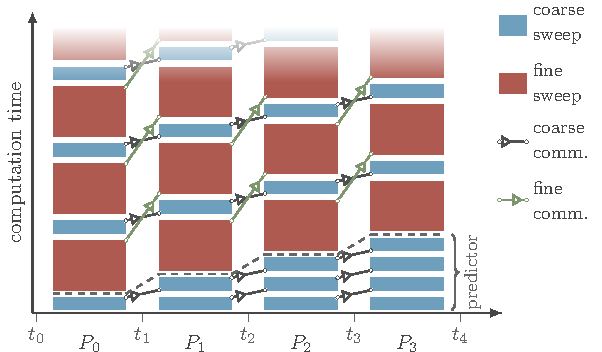
\includegraphics[width=\textwidth]{images/pfasst_diagram.pdf}
  \caption{Representation of the PFASST method using two levels. Created using pfasst-tikz \protect\footnotemark.}
\end{figure}
% END: ensure it's on the same page as the picture
\footnotetext{\url{https://github.com/f-koehler/pfasst-tikz}}

With \(K_s\) denoting the number of SDC iterations needed to compute the solution to the desired accuracy in serial using the fine nodes, and \(K_p\) denoting the number of PFASST iterations for the same accuracy, the parallel efficiency of PFASST is bounded by \(E < K_s/K_p\). That is, when compared to standard Parareal with SDC propagators (\(E < 1/K_p\)), the bound is relaxed by a factor of \(K_s\).

\section{LibPFASST} \label{sec:libpfasst_usage}

Proper implementation of numeric methods is time-consuming and error prone. This chapter presents a simplified overview of the building blocks of the PFASST scheme, but omits the more complex mathematical aspects an implementation must account for. Additionally, parallel programs are notoriously hard to validate. These factors come together to make an efficient, reliable implementation of the PFASST method particularly hard to accomplish. For a user wanting to apply PFASST (or one of the other schemes mentioned in this section) to the solution of a specific problem, or even to implement a modified version of a method, it is better to start from a known, reliable open-source implementation.

LibPFASST \cite{libpfasst_github} is an implementation of the PFASST algorithm, written in Fortran 2008 using MPI for parallelization. It offers, through different configurations, support for all the methods previously described, as well as a number of additional variations of PFASST components which aren't mentioned here. It structured in a modular and extensible way, facilitating mixing and matching of different PFASST components and user-created components, and optionally integrates with other libraries such as PETSc, AMReX and Sundials.

Here we aim to provide a simplified introduction to the usage of LibPFASST, which will be useful in illustrating details of the cpfasst implementation. For a  complete user's guide to LibPFASST, refer to \cite{libpfasst_ug}. This description is based on the tutorial \ilc{EX2_Dahlquist}, included with the LibPFASST source code.

The usage of LibPFASST to solve a simple problem involves the steps below:

\begin{itemize}
    \item \textbf{Configure LibPFASST parameters:} LibPFASST has a few mandatory parameters, and several optional ones. These include tolerances, number of levels and sweeps per level, number and type of nodes, and several others - a comprehensive guide is provided in \cite{libpfasst_ug}. The configuration is stored in an instance of the main LibPFASST structure, \ilc{pf_pfasst_t}, and can be initialized and changed through any combination of nml file parameters, command line parameters, and writing to the \ilc{pf_pfasst_t} structure in user code.

    \item \textbf{Choose (or define) a data encapsulation:} Choose a type to represent a single instance of the solution over the space domain for one level. LibPFASST provides several such types to choose from, e.g. \ilc{pf_ndarray_t}, which implements an n-dimensional array of real numbers. Alternatively, a custom encapsulation can be implemented by the user, by extending type \ilc{pf_encap_t}, and defining its deferred type-bound procedures, which are used to operate on the encapsulated data (e.g. \ilc{norm}, \ilc{axpy}). The data encapsulation must be paired with a compatible factory to create and destroy the encapsulation type, which is provided for the predefined encapsulations, but can also be customized by the user through a type extending \ilc{pf_factory_t}.

    \item \textbf{Define a user level:} The user must define a type extending \ilc{pf_user_level_t}, and implementing its deferred type-bound procedures \ilc{restrict} and \ilc{interpolate} for the chosen encapsulation. Those are invoked by LibPFASST for the multi-level spatial restriction and interpolation operations. FAS correction is handled automatically by LibPFASST. 

    \item \textbf{Define a sweeper:} The user must define a type expanding one of the LibPFASST sweeper types, and implementing any deferred type-bound procedures contained in that sweeper. Each of the sweeper types is suitable to the solution of problems of a certain form, and these procedures are used for problem-specific evaluations in the given form. In the case of the implicit-explicit sweeper used in this project, suitable for problems of the form \(y'=f_1(y,t)+f_2(y,t)\), where \(f_1\) is treated explicitly and \(f_2\) implicitly, the procedures to be defined are:
    \begin{itemize}
        \item \ilc{f_eval}: Evaluate the requested piece of the right-hand side function (\(f_1\) or \(f_2\)) for the provided time \(t\) and approximate solution \(y\).
        \item \ilc{f_comp}: Implicitly solve the equation \(y-dtq*f_2(y,t)=rhs\) for the provided time \(t\), approximate solution \(y\), right-hand side value \(rhs\), and \(dtq\in\mathbb{R}\).
    \end{itemize}
\end{itemize}
% !TEX root = ../main.tex
\chapter{Interoperability between C and Fortran}
\label{chapter:interoperability}

\textbf{Note on definitions:} For the purposes of this work, a \textit{processor} is defined according to the Fortran standard \cite{adams2008fortran}: the combination of a compiler and the computing system used for program execution. Additionally, \textit{procedure} is used as a general term to refer to Fortran functions and subroutines, as well as C functions.

Interoperability with Fortran is a challenging prospect, due to how the Fortran standard is written: it is permissive by design. The standard specification is limited to \cite{F90standard,F2003standard,F2018standard}: 

\begin{itemize}
	\item the forms that a program written in the Fortran language can take,
	\item the rules for interpreting the meaning of a program and its data,
	\item the form of the input data to be processed by such a program, and
	\item the form of the output data resulting from the use of such a program.
\end{itemize}

Any aspect not covered by the standard is considered to be processor-dependent, and is left up to its implementation. Processors are also considered standard-conforming even when implementing features not described in the standard. This allows for greater experimentation and development of the language, with successful features becoming candidates for inclusion in the standard on future versions, but also requires the programmer to know about and avoid those extra features when portability is desirable \cite{adams2008fortran}. In addition to this, the AMD64 ABI (Application Binary Interface) explicitly states that a formal Fortran ABI is neither provided or desirable, as it would hinder a compiler's ability to optimize for high performance applications on its target system \cite{x86_64_abi}. Some guidelines are provided for Fortran 77--compatible features in the interest of interoperability, but each compiler implementation is otherwise free to do as they see fit.

However, as mentioned in \refChapter{chapter:introduction}, there is significant demand for the reuse of Fortran code, especially in the scientific computing community, and often from code written in a different language. The Fortran 2003 standard addresses this by the introduction of a standardized interoperability interface between Fortran and C. The choice of C is not incidental: aside from all Fortran 77-compatible features having a direct equivalent in C, C is recognized as a ``lingua Franca'' of programming languages \cite{adams2008fortran}. A number of other programming languages support interoperability with C, including scientific computing staples MATLAB, C++, Python, and R, and support for C interoperability in Fortran indirectly allows any such language to also interoperate with Fortran. Interestingly enough, it also provides the only standard means of interoperability between binaries from different Fortran compilers --- though in this case it is preferable to simply recompile the code.

While the use of Fortran 2003 interoperability features precludes many of the challenges in C integration, looking at how C/Fortran interoperable programs were built before those features were introduced provides significant insight into the similarities and differences between C and Fortran, and illustrates some of the challenges introduced by interoperability in general. \refSection{sec:interop_f90} provides an overview of C/Fortran interoperability mechanisms using only Fortran 90 features. \refSection{sec:interop_f03} introduces the Fortran 2003 C interoperability features, and how they address previous issues.

This analysis is restricted to the implementation of correct calls to procedures between the two languages. While interoperable access between Fortran \ilc{common} blocks and C global variables is defined in the Fortran 2003 standard, the use of those features often discouraged as a bad programming practice even in single-language environments \cite{clerman2011modern}, so aspects of interoperability exclusive to their use will not be discussed here.

\section{Fortran 90} \label{sec:interop_f90}

\textbf{An important \textit{caveat}:} as this section will demonstrate, interoperability between C and Fortran 90 relies heavily on processor-dependent behavior, and as such there can be no expectation of portability. The code examples provided were tested using the GNU Compiler Collection version 10.1.0, targeting the x86-64 Linux GNU platform, and may require adjustments for any other environment. It is important to read this section not as a tutorial, but as a guide to important aspects of compatibility that must be considered when developing multi-language applications. Use of the standard interoperability features described in \refSection{sec:interop_f03} is strongly recommended over the techniques shown here.

Fortran standards prior to 2003 did not offer standardized support for interoperability with C. However, the two languages are linked for historical reasons, with the first complete Fortran 77 compiler \cite{feldman1985portable}, \textit{f77}, using the second pass of a C compiler as a code generator \cite{feldman1979implementation}, establishing the groundwork for C representations of Fortran types, and compatibility between equivalent Fortran and C procedure calls. This equivalence goes so far as to enable automated conversion of Fortran 77 source code (even extending into some Fortran 90 features) into C \cite{feldman1990fortran}. 

Ensuring correctness for a procedure call between C and Fortran is at a low-level no different from ensuring correctness for a procedure call between two different compiling units in either of the two languages. The practical difference arises from the fact that in a single-processor environment, the user need not be concerned with (or, in most cases, even aware of) most of those aspects, as the compiler and linker will handle them automatically.

In general, the requirements for an interoperable procedure call can be summarized as:
\begin{enumerate}
	\item \textbf{Data types must be correctly defined wherever the data is accessed:} A simplistic interpretation of this requirement is that both the caller and callee must have matching definitions of the data types in the procedure's arguments and return values. That need not be the case, though: if a type is not accessed in the callee context, but a data of that type is passed as an argument for architecture reasons, or in order to be forwarded to a different procedure call, there is no need to provide the callee with a definition of the type (it is then considered opaque to the callee). On the other hand, consider a C pointer passed as an argument to a C function which accesses the referenced data: it is not sufficient for the function to understand how a C pointer is defined, it also needs a definition for the data it references.
	\item \textbf{Caller and callee must have the same interpretation of a procedure:} In a single-compiler environment, this is guaranteed as long as both reference the procedure by the same syntax. In multi-language programs, complications can arise from different argument and return value passing conventions, or different call sequences. Some interoperability tools, such as language bindings, will automatically handle this. In cases where such a tool isn't available (as is the case between Fortran 90 and C), the developer must be aware of the inner workings of both compilers in order to insure this.
\end{enumerate}

\subsection{Intrinsic data types} \label{sec:interop_f90_intrinsic}

While the Fortran standard defines only five intrinsic types (\ilc{integer}, \ilc{real}, \ilc{complex}, \ilc{character}, and \ilc{logical}), it is possible, through the use of type parameters, to create an arbitrary number of standard-complying primitive types. The default parameters, and the underlying data representation, are processor-dependent. While a number of sources defining built-in type mappings between C and Fortran is readily available on the internet, they often do not include information on which compilers and platforms they apply to, making their use unreliable. Documentation from the compiler and/or platform can be used to determine proper type mappings, but a popular alternative is to run test code to comparing different data types in each language until the desired match is found. The x86-64 guidelines for Fortran 77--compatible types, which are followed by GCC, recommend the use of the type mappings provided by \textit{g77} \cite{x86_64_abi}, some of which are shown in \refTable{tab:f90types}.

\begin{table}
	\centering
	\begin{tabular}{|c|c|c|}
		\hline 
		Fortran 77 & Fortran 90 & C \\
		\hline 
		\hline 
		\ilc{INTEGER*4} 	& \ilc{integer(kind=4)} 	& \ilc{int} \\
		\hline 
		\ilc{INTEGER*8} 	& \ilc{integer(kind=8)} 	& \ilc{long int} \\
		\hline 
		\ilc{REAL*4} 		& \ilc{real(kind=4)} 		& \ilc{float} \\
		\hline 
		\ilc{REAL*8}		& \ilc{real(kind=8)} 		& \ilc{double} \\
		\hline 
		\ilc{COMPLEX*4} 	& \ilc{complex(kind=4)} 	& \ilc{float _Complex} \\
		\hline 
		\ilc{COMPLEX*8} 	& \ilc{complex(kind=8)} 	& \ilc{double _Complex} \\
		\hline 
		\ilc{LOGICAL}		& \ilc{logical} 			& \ilc{signed int} \\
		\hline
		\ilc{CHARACTER} 	& \ilc{character} 			& \ilc{char[]} \\
		\hline 
	\end{tabular}
	\caption{Mapping between Fortran 77--compatible types and C built-in types for the x86-64 platform. Adapted from \cite{x86_64_abi}.}
	\label{tab:f90types}
\end{table}

Most of the type mappings are straightforward, but the two non-numeric types warrant specific discussion: 
\begin{itemize}
	\item In standard C, relational, equality and logical operators return \ilc{0} for \textit{false} and \ilc{1} for \textit{true}, while conditional statements consider a value \textit{false} when it is equal to zero, and \textit{true} otherwise \cite{C11standard}. Meanwhile, the underlying representation of Fortran's \ilc{logical} values \ilc{.true.} and \ilc{.false.} is processor-dependent. For interoperability, it is important to ensure a match not only in the underlying representation, but also in the values.
	\item C expects character strings to be terminated by a \ilc{null} character, but Fortran makes no such guarantee, so care must be taken when processing a string created by Fortran in a C environment. Additionally, Fortran \ilc{character} strings often modify a procedure's call signature when passed as arguments. This is further discussed in \refSection{sec:interop_f90_strings}.
\end{itemize}

\subsection{Procedure arguments and returns} \label{sec:interop_f90_calls}

One of the fundamental differences between C and Fortran relates to argument passing conventions: in C, function arguments are always passed by value (what is referred to by C programmers as ``passing by reference'' is in fact passing a pointer argument by value). Meanwhile, the Fortran 90 standard leaves the mechanism of argument passing entirely up to the implementation, but the behavior it defines is that of passing by reference, except for dummy arguments with the \ilc{intent(in)} attribute. In the interest of maintaining backwards compatibility with Fortran 77, which does not support the \ilc{intent} attribute, Fortran compilers usually pass all formal arguments by reference through a C-style pointer, and any additional compiler-generated arguments either by value or reference. To accommodate this difference, the C implementation must be adjusted to always take pointers to the desired argument values, instead of the values themselves, and dereference them on use. The source code in \ref{src:f90_calls} illustrates this in both directions.

\begin{listing}
	\inputminted{C}{src/f90/calls/csrc.c}
	\inputminted{Fortran}{src/f90/calls/fsrc.f90}
	\caption{Example of interoperable procedure calls between Fortran 90 and C code, using GNU Fortran 10.1.0 in the x86-64 platform.}
	\label{src:f90_calls}
\end{listing} 

Function return values in Fortran behave as if passed by value, but their actual behavior is processor-defined and often involves the result value as a hidden argument, appended by the compiler to the function signature. gfortran utilizes a hidden result values for functions returning arrays or the \ilc{character} type \cite{gfortranmanual}. If possible, it is best to avoid this issue entirely by restricting interfaces to Fortran subroutines, which are equivalent to C functions with \ilc{void} return type, and add a parameter to the function (which on the Fortran side should be either \ilc{intent(out)} or \ilc{intent(inout)}) for any data to be passed from the callee to the caller. This does not, however, preclude the addition of hidden arguments by the Fortran compiler for different reasons --- one common example is shown in \refSection{sec:interop_f90_strings}.

It is important to note that while matching symbol names (discussed in \refSection{sec:interop_f90_names}), argument passing conventions and data type definitions is usually sufficient for correct interoperable calls, it is possible (and at least for x86-64, allowed) that the Fortran compiler does not comply with the platform's C calling convention at all. In this case, a deeper analysis is needed to find which calling conventions are supported on both sides, and whether the calling convention can be modified through compiler directives or flags.    

\subsection{Symbol names} \label{sec:interop_f90_names}

When linking binaries originating from a single compiler, matching symbol names between different compilation units is not a concern --- as long as the code is correct, the symbol name resolution process is transparent to the user. In multi-language programming there is often need for user input in this process. A common use case is interoperability between C and C++ compilers: while the two languages are close in syntax, they use different symbol name decoration and mangling schemes, so a naive implementation will cause a mismatch in symbol names. In this case the solution is simple: declaring a function with the modifier \ilc{extern "C"} tells the compiler to use a C-style symbol for that function. In the case of C and Fortran 90, however, no such mechanism is available: the developer must understand the symbol name decoration schemes for each of the compilers involved, and name their procedures such that both sides will refer to the resulting symbol by the same name. It is likely that this results in the same procedure being referred to by similar but different names in either language. It is important to highlight that these name decoration schemes are expected to change between platforms for C, and between platforms, compilers, or even compiler versions for Fortran, and can also be affected by compiler flags and directives \cite{gfortranmanual}. This makes symbol names a major issue when it comes to interoperability.

The code in \refSrc{src:f90_calls} illustrates symbol name decoration for this processor: C functions produce symbols with no added decoration, while external Fortran procedures produce symbols in lowercase, with one trailing underscore (ignoring the ABI's guideline \cite{x86_64_abi} of two trailing underscores for names containing an underscore). For this scenario, reconciling C and Fortran names is simple: use only lowercase names and append an underscore to names of interoperable procedures on the C code. Alternatively, GNU Fortran's \ilc{-fno-underscoring} flag can be used to modify the behavior --- the lowercase restriction remains, as Fortran syntax is case-insensitive. Fortran functions inside modules (not illustrated in this section) follow a more complex, processor-specific mangling scheme.

\subsection{Arrays and array descriptors} \label{sec:interop_f90_arrays}

A widely known difference between C and Fortran relates to the storage of multidimensional arrays: C utilizes a row-major layout, and Fortran a column-major one. In both cases the layout is fixed by the standard, and correct interoperable access of a multidimensional array created by the other language requires inverting the order of array subscripts. C subscripts are zero-indexed, while Fortran subscripts are one-indexed, and any subscripts passed as arguments should be adjusted to reflect that.

\textit{Efficient} interoperable access, however, is a different matter, as simply inverting the subscripts will often break spatial locality and result in cache-unfriendly code. Efficient access requires either changing the code to optimize for the other language's layout or converting between layouts through an auxiliary copy of the array. When feasible, it is best to avoid this scenario entirely and access the data only in one language.

C and Fortran generally pass array arguments in a similar manner, through the address of the first array element. The following restrictions apply:
\begin{itemize}
	\item The entire array must be stored in contiguous memory. In Fortran 90 that is guaranteed by the standard, but in C, dynamically allocated multidimensional arrays are sometimes implemented a list of pointers to row data --- this layout is not interoperable unless data for the rows is contiguous, in which case a pointer to the start of the data, not to the pointer list, must be passed.
	\item For Fortran procedures, interoperability of array arguments depends on how they are declared. This is illustrated in \refSrc{src:f90_arrays}.
		\begin{itemize}
			\item \textit{Explicit-shape array} dummy arguments are interoperable with a C array of the same total size;
			\item \textit{Assumed-size array} dummy arguments are interoperable with a C array. Array dimensions can be passed as separate arguments as needed;
			\item \textit{Assumed-shape} dummy arguments are not interoperable. Fortran procedures containing these arguments expect a pointer not to the first element, but to a compiler-dependent descriptor, further discussed in \refSection{sec:interop_f90_derived}.
		\end{itemize}
\end{itemize}

\begin{listing}
	\inputminted{C}{src/f90/array_types/csrc.c}
	\inputminted{Fortran}{src/f90/array_types/fsrc.f90}
	\caption{Fortran 90 and C code illustrating how different array dummy arguments affect interoperability. Though the actual argument is the same, use of an assumed-shape dummy argument changes the low-level mechanism for argument passing, causing the C function incorrectly interpret that argument.}
	\label{src:f90_arrays}
\end{listing}

\subsection{Strings} \label{sec:interop_f90_strings}

As mentioned in \refSection{sec:interop_f90_intrinsic}, treatment of character strings differs significantly between the two languages. C does not have a native string type. By convention, and following the behavior of the standard C functions for string handling \cite{C11standard}, a C string is a \ilc{char} array terminated by the \ilc{NULL} (\ilc{'\0'}) character. A C function operating on a string typically takes only a pointer to the start of the array as argument, and is not explicitly aware of its length --- the string is instead considered to extend until the \ilc{NULL} terminator.

Meanwhile, Fortran strings are of intrinsic type \ilc{character}, with length specified by the \ilc{len} type parameter, and unused space being padded with blank (\ilc{' '}) characters. A procedure taking a character string as a dummy argument can specify an explicit or assumed-length parameter. Assumed-length dummy arguments will automatically adapt to the actual argument used for the call, while explicit length dummy arguments will cause an actual argument of higher length to be truncated. Implementation of this behavior is processor-dependent, but most compilers use the convention established by f77: a pointer to the character string is passed as an argument at the position of the dummy argument, and a pass-by-value \ilc{integer} hidden argument is appended to the end of the argument list, containing the length of the string and passed by value. If multiple string dummy arguments are present, their length hidden arguments are appended in the order of their appearance in the argument list. In GNU Fortran, the length of the actual argument is passed as a hidden argument regardless of how the dummy argument length is specified, but ignored for dummy arguments of explicit length.

When designing a C function to be called from Fortran, the additional argument can be read as a C \ilc{int} at the correct position. If the Fortran string is used as an argument to any C functions that do not take a length argument, a \ilc{NULL} terminator should first be appended to avoid out-of-bounds access issues. When calling a Fortran function from C, the string length hidden argument must be correctly passed, its value being the string length as returned by the C function \ilc{strlen}.

A great example of how reliance on processor-specific behavior for interoperability can cause issues is related to this mechanism: in 2019, a GNU Fortran update broke a number of C applications that omitted the hidden argument in BLAS/LAPACK calls for single-character strings, including CBLAS and LAPACKE. An unrelated bug fix exposed this issue, which had been carried on between implementations from decades, eventually prompting the compiler to add a flag to disable the bug fix due to the number of applications affected \cite{kalibera2019gfortran,corbet2019scstrings}.

\subsection{Derived data types} \label{sec:interop_f90_derived}

Type-shadowing is the creation of an equivalent representation for a derived type in a different language, allowing correct access to the data contained in variables of that type. A Fortran \ilc{type} can be shadowed by a C \ilc{struct}, and vice-versa, with the following restrictions\cite{pletzer2008exposing}:

\begin{itemize}
	\item All members must be of interoperable types (including members of derived types); 
	\item The Fortran \ilc{type} must have the \ilc{sequence} attribute to prevent the compiler from reordering members in memory;
	\item If the Fortran and C compilers use different rules for structure padding, manual padding or packing may be required;
\end{itemize}

The main challenge lies in fulfilling the first condition, in particular for numerical applications using modern Fortran features. As mentioned in \refSection{sec:interop_f90_arrays}, assumed-shape array dummy arguments are not interoperable, as they are wrapped in an opaque descriptor by the Fortran compiler. This also applies to assumed-shape type members, and additionally applies to members with the \ilc{allocatable} or \ilc{pointer} attributes. In order for those members (and thus the type) to be interoperable, the C code must be capable to interpret the processor-dependent Fortran descriptors, which are not documented and, for closed-source compilers, must be reverse-engineered. The CHASM Language Interoperability Tools \cite{rasmussen2001chasm} project provides a C interface to Fortran array descriptors for different compiler vendors, but is no longer maintained.

Even if the goal is to treat members of non-interoperable types as opaque, while maintaining access to members of interoperable types, defining a shadowing type can be difficult. The size of the descriptors varies between compiler vendors and platforms, as shown in \refTable{tab:f90descriptors}. Even with the introduction of standardized C interoperability features by Fortran 2003, there is no mechanism allowing a reliable implementation of type-shadowing for types containing descriptor-based members. In 2012, a technical specification was released defining standardized C descriptors for assumed-shape, assumed-rank, and deferred-shape arrays, including allocatables and pointers --- as of GNU Fortran version 10.1.0, it remains not fully supported \cite{gfortranmanual}.

\begin{table}
	\centering
	\begin{tabular}{|c|c|c|c|}
		\hline 
		Processor & \ilc{array(:)} & \ilc{array(:,:)} & \ilc{array(:,:,:)} \\
		\hline 
		\hline 
		gfortran 4.1.2 i686 	& 24 & 36 & 48 \\
		\hline 
		gfortran 4.1.1 x86\_64 	& 72 & 96 & 120 \\
		\hline 
		ifort 10.1 i686 		& 48 & 60 & 72 \\
		\hline 
		ifort 9.1.041 ia64		& 96 & 120 & 144 \\
		\hline 
	\end{tabular}
	\caption{Size in bytes of derived types with a pointer array member of rank 1, 2 and 3. Adapted from \cite{pletzer2008exposing}}
	\label{tab:f90descriptors}
\end{table}



\section{Fortran 2003} \label{sec:interop_f03}

In light of all the previously mentioned issues with interoperability in earlier standards, the Fortran 2003 standard introduced standardized support for interoperability with C. The interoperability features in this standard do not introduce much in the way of new solutions, but rather formalize what was previously known to work with most Fortran 90 compilers \cite{pletzer2008exposing}. Still, having those features as part of the standard allows something that was previously impossible: portability. Any standard-compliant interoperable interfaces are guaranteed to work between a processor implementing the Fortran 2003 standard and one of its companion processors.

The standard defines a \textit{companion processor} as a processor-dependent mechanism by which global data and procedures may be referenced or defined \cite{F2003standard}. This is not necessarily a C compiler, but any processor capable of working with data and procedures described in terms of C (e.g. a C++ compiler). To comply with the Fortran 2003 standard, a Fortran processor must define at least one companion processor --- which can be itself. The Fortran processor is not required to correctly interoperate with any processor it does not explicitly define as a companion. For Fortran processors defining multiple companions, the means of selecting between them are processor-dependent.

Standard interoperability can be summarized by two major features:
\begin{itemize}
	\item The \textbf\texttt{iso\_c\_binding} intrinsic module provides named constants, derived data types, and module procedures supporting interoperability;
	\item The \textbf\texttt{bind(C)} attribute, applicable to procedures and derived types, marks a Fortran element as interoperable with C. This triggers the Fortran processor to adjust its low-level representation of that element, ensuring compatibility with the companion processor, but also imposes some restrictions on what the element may contain.
\end{itemize}

This section details how the previously described approach to interoperability for Fortran 90 code is affected by the use of these features.

\subsection{Intrinsic data types} \label{sec:interop_f03_intrinsic}

As discussed in \refSection{sec:interop_f90_intrinsic}, the question of interoperability between C and Fortran intrinsic types is largely one of determining the correct \ilc{kind} type parameters to match each C type for a given processor. This issue is solved in a portable manner through the use of the kind parameter constants defined by the \ilc{iso_c_binding} intrinsic module, which are guaranteed to match the companion processor's implementation of a given C type. \refTable{tab:f03types} shows a small sample of the available constants and their correspondence with intrinsic C types. Contrasting it to \refTable{tab:f90types} reveals an additional benefit of the use of these constants: since they are named after their C equivalents, readability of interoperable Fortran types is improved, as design intention of the choice of kind value is clearly communicated. This, in turn, facilitates equivalency between references to the type in Fortran and C. 

\begin{table}
	\centering
	\begin{tabular}{|c|c|}
		\hline 
		Fortran type & C type \\
		\hline 
		\hline 
		\ilc{integer(kind=c_int)}				& \ilc{int} \\
		\hline 
		\ilc{integer(kind=c_long)}				& \ilc{long int} \\
		\hline 
		\ilc{real(kind=c_float)} 				& \ilc{float} \\
		\hline 
		\ilc{real(kind=c_double)}				& \ilc{double} \\
		\hline 
		\ilc{complex(kind=c_float_complex)} 	& \ilc{float _Complex} \\
		\hline 
		\ilc{complex(kind=c_double_complex)} 	& \ilc{double _Complex} \\
		\hline 
		\ilc{logical(kind=c_bool)}				& \ilc{_Bool} \\
		\hline
		\ilc{character(kind=c_char)} 			& \ilc{char} \\
		\hline 
	\end{tabular}
	\caption{A sampling of \ilc{iso_c_binding} kind parameter constants and their correspondent C types \cite{F2003standard}.}
	\label{tab:f03types}
\end{table}

As with Fortran 90, interoperabilty of \ilc{logical} and \ilc{character} warrants additional observations: 
\begin{itemize}
	\item The \ilc{logical(c_bool)} type is guaranteed to interoperate with C99's \ilc{_Bool} type, for which the C standard defines the values \ilc{true} as 0 and \ilc{false} as 1. However, for the reasons mentioned in \refSection{sec:interop_f90_intrinsic}, it is common in C code to use variables of integer type to storage of boolean values, and to consider any value non equal to zero as \ilc{true}. Such representations are not interoperable, and should be cast into \ilc{_Bool} types for interoperable use \cite{gfortranmanual}.
	\item The \ilc{character(c_char)} type is only considered interoperable when its length is fixed and equal to 1. This changes the representation of interoperable strings, which must now be defined by Fortran as an array. Treatment of strings in this scenario is detailed in \refSection{sec:interop_f03_strings}.
\end{itemize}

Two derived Fortran types are defined by the \ilc{iso_c_binding} module: \ilc{c_ptr} is interoperable with a C data pointer, and \ilc{c_funptr} is interoperable with a C function pointer. Used in conjunction with the module functions \ilc{c_loc} (which returns a \ilc{c_ptr} containing the address of a Fortran variable) and \ilc{c_funloc} (which returns a \ilc{c_funptr} containing the address of a Fortran procedure), these types provide full interoperability with C pointers.

\subsection{Procedures} \label{sec:interop_f03_calls}

A Fortran procedure is considered interoperable if it has the \ilc{bind(C)} attribute. This applies both to procedures defined in Fortran to be callable from C, and to procedures declared in a Fortran interface block and defined in C --- as shown in \refSrc{src:f90_arrays}, the interface defines how Fortran invokes a procedure. A \ilc{bind(C)} procedure is considered interoperable, and must obey a set of restrictions enforced by the compiler. Included in those conditions are \cite{adams2008fortran}:
\begin{itemize}
	\item Each dummy argument of an interoperable procedure must be an interoperable variable or an interoperable procedure. This excludes arguments with the \ilc{allocatable} and \ilc{pointer} attributes, assumed-shape arrays, and \ilc{character} types with length other than 1. Aside from character strings, these were known restrictions for interoperability with Fortran 90, as discussed in \refSection{sec:interop_f90}, which the standard makes official.
	\item The result variable of an interoperable function procedure or interface must be an interoperable scalar variable. This precludes the issues discussed in \refSection{sec:interop_f90_calls} with some return types are implemented by Fortran compilers as hidden arguments.
\end{itemize}

A Fortran procedure with the \ilc{bind(C)} attribute is guaranteed to be interoperable with a C function prototype if the conditions below are met \cite{F2003standard}:
\begin{itemize}
	\item If the Fortran procedure is a subroutine, the C function must have a return type of \ilc{void}. If it is a function, the return types of both functions must be interoperable;
	\item Each argument in the C function corresponds directly to the Fortran dummy argument in that position, and:
		\begin{itemize}
			\item If the Fortran dummy argument has the \ilc{value} attribute, the C function argument and the Fortran dummy argument are of interoperable types;
			\item Otherwise, the C function argument is a pointer referencing an entity interoperable with the Fortran dummy argument type;
		\end{itemize}
\end{itemize}

With the previous conditions met, the Fortran processor is guaranteed to generate a low-level representation of the procedure interface consistent with the companion processor's low-level representation of the C function prototype. This includes correct matching of the companion processor's calling convention, precluding the related issues mentioned in \refSection{sec:interop_f90_calls}.

When applied to a procedure, the \ilc{bind(C)} statement generates a \textit{binding label}, which determines the name by which it can be referred to in C code. A case-sensitive binding label can be specified in the bind statement (\ilc{bind(C, name="BindingLabel")}), and is independent of the procedure name in Fortran. If a binding label is not explicitly defined, the lowercase name of the Fortran procedure is used. Binding labels are required to be unique in a Fortran program. For cases where it is desirable to declare an interoperable procedure interface without an unique global identifier (e.g. when specifying the type of a procedure pointer), an empty label can be specified in the \ilc{bind} statement.

\begin{listing}
	\inputminted{C}{src/f03/calls/csrc.c}
	\inputminted{Fortran}{src/f03/calls/fsrc.f90}
	\caption{Example of interoperable procedure calls between Fortran and C code, using the Fortran 2003 standard interoperability features.}
	\label{src:f03_calls}
\end{listing}

\refSrc{src:f03_calls} illustrates interoperability of the same functions as \refSrc{src:f90_calls}, with the use of standard interoperability features. The \ilc{bind(C)} procedures are referenced by the same names in both languages --- a property that also applies if they are defined inside a Fortran module. If a \ilc{bind(C)} procedure does not fit the restrictions for interoperability, a compiler error is generated: adding a \ilc{bind(C)} label to the interface procedure in \refSrc{src:f90_arrays} will cause it to not compile unless the assumed-shape array dummy argument is removed.

\subsection{Derived data types and arrays} \label{sec:interop_f03_derived}

The mechanism of interoperability for derived data types is similar to procedures: to be considered interoperable, a type must have the \ilc{bind(C)} attribute, and all its members must be of interoperable types. Additionally, such a type may not use object-oriented Fortran features, such as the \ilc{extends} attribute or type-bound procedures. Use of the \ilc{sequence} attribute, recommended in \refSection{sec:interop_f90_derived}, is also forbidden: it is, however, not relevant here, as the resulting type is guaranteed to match the companion processor's representation of an equivalent C \ilc{struct}. The restrictions discussed in \refSection{sec:interop_f90_derived} still apply, as \ilc{allocatable}, \ilc{pointer}, and assumed-shape types are not considered interoperable, and as such cannot be members of an interoperable type.

Interoperability for arrays remains the same as described in \refSection{sec:interop_f90_arrays}. Assumed-shape and deferred-shape arrays, previously known to not be interoperable, are now explicitly disallowed as dummy arguments to interoperable procedures and members of interoperable derived types, as are Fortran 2003's assumed-rank arrays.

\subsection{Strings} \label{sec:interop_f03_strings}

As mentioned in \refSection{sec:interop_f03_intrinsic}, the \ilc{character(c_char)} type is only considered interoperable when used with a fixed length equal to 1. As a consequence of this restriction, an interoperable string is represented in Fortran as it is in C: a 1D array of type \ilc{character(c_char)}. Fortran's rules of sequence association allow a dummy argument this type to be associated with an actual argument that is a Fortran-style string \cite{F2003standard}, but the user still needs to be aware of the differences in string conventions when it comes to null-termination vs blank padding, and convert between them accordingly. An example of this use is shown in \refSrc{src:f03_strings}.

\begin{listing}
	\inputminted{C}{src/f03/strings/csrc.c}
	\inputminted{Fortran}{src/f03/strings/fsrc.f90}
	\caption{Use of interoperable strings in a C function called from Fortran, in accordance with the Fortran 2003 standard. Sequence association rules allow a Fortran string actual argument to be associated with the interoperable character array dummy argument. Adapted from \cite{F2003standard}.}
	\label{src:f03_strings}
\end{listing}
% !TEX root = ../main.tex
\chapter{Architecture and implementation of the interface}
\label{chapter:implementation}

\section{Scope and design goals} \label{sec:impl_design_goals}

The goal for this work is to design cpfasst, an interface allowing the use of LibPFASST entirely from C code. This not only enables use of LibPFASST by users unfamiliar with Fortran, but, as discussed in \refChapter{chapter:interoperability}, can be accessed from any language that can interoperate with C, opening the doors for reuse from C++, Python and R, for example. Goals for the design were established early on and refined during development, and can be summarized as follows:
\begin{itemize}
    \item \textbf{Portability:} As discussed in \refChapter{chapter:interoperability}, portability can pose a significant challenge for code relying on C/Fortran interoperability. The goal for cpfasst was to impose as few restrictions on the portability of LibPFASST as possible: ideally, any system capable of building and running LibPFASST should, with the addition of a companion C compiler, build and run cpfasst.

    \item \textbf{Maintainability:} LibPFASST continues to be developed, and as such the implementation of its components is subject to change. To mitigate the risk of changes to LibPFASST breaking the C interface, it should rely as little as possible on specifics of the LibPFASST implementation. Additionally, whenever possible, cpfasst should test aspects of the LibPFASST implementation it relies on, with any breaking change causing cpfasst to fail during verification, not during use.

    \item \textbf{Performance:} The cpfasst interface should impose minimal performance and memory overhead on the LibPFASST main loop.

    \item \textbf{Reliability:} Use of LibPFASST through the C interface should be as reliable as with Fortran. Code developed for the interfaces should follow best practices for the language it is implemented in, and be thoroughly verified.

    \item \textbf{C-only interface:} The implemented interface should assume only familiarity with C, and any aspects that cannot be changed to be intuitive to users unfamiliar with Fortran should be highlighted and well-documented.
\end{itemize}

Overall, the goal is to afford the C user as much of the flexibility in use of the Fortran user as possible, while meeting the goals above. The interface is developed for the LibPFASST components required for usage as described in \refSection{sec:libpfasst_usage}, with all problem-specific code being developed in C. Specifically, we targeted reproduction of the tutorial code distributed with LibPFASST from a C implementation.

\section{LibPFASST architecture} \label{sec:libpfasst_arch}

A summary of the elements of LibPFASST usage was presented in \refSection{sec:libpfasst_usage}, but to understand the challenges related to the creation of the interoperable interface, we must first take a closer look at the underlying implementation. As mentioned in the summary, at the core of LibPFASST library is a single derived type, \ilc{pf_pfasst_t}, containing all data related to configurations and working variables for a PFASST run. \refFigure{fig:libpfasst_types} shows a hierarchy of the derived types under \ilc{pf_pfasst_t}, providing a general overview of the entire data structure. Examining this hierarchy is useful for understanding which LibPFASST types are candidates for, or require, user extension. 

\begin{figure}[ht]
  \centering
  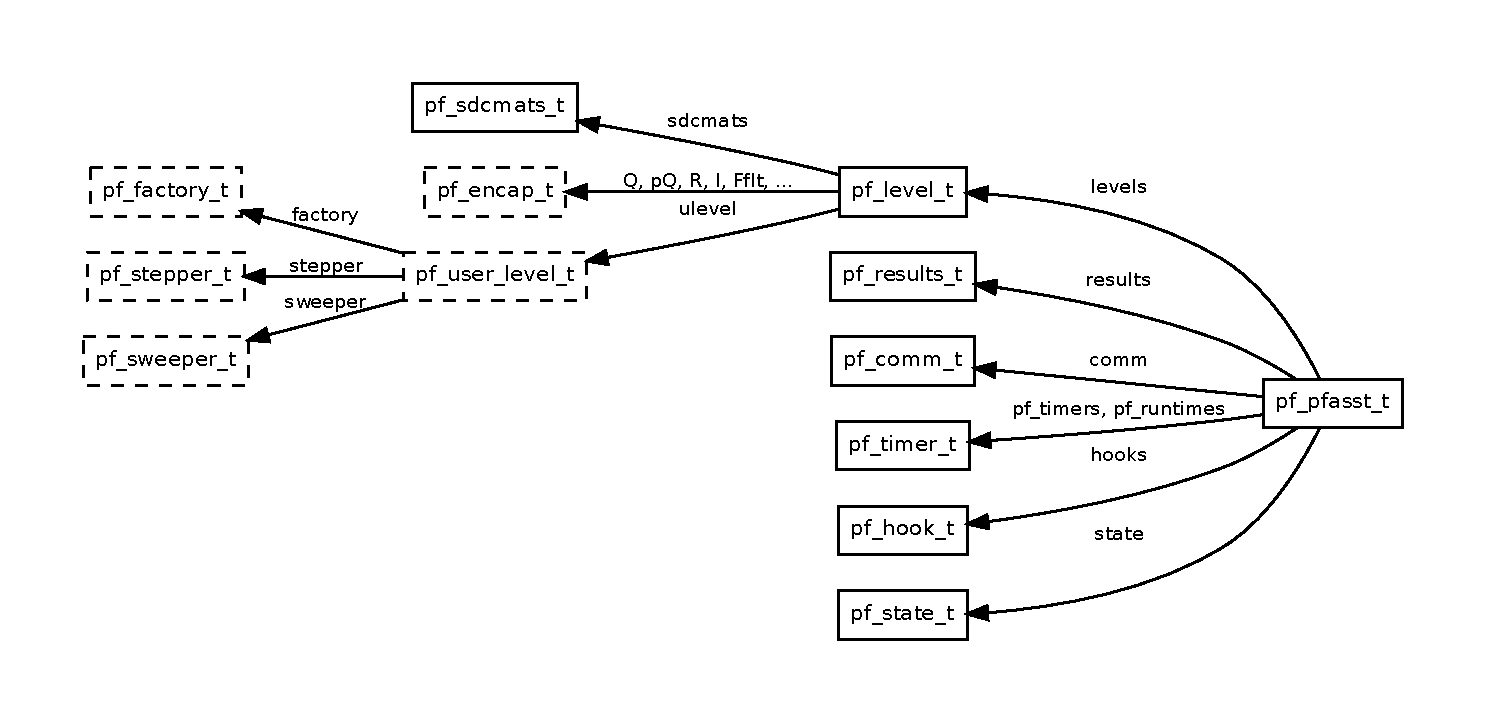
\includegraphics[width=\textwidth]{images/pf_pfasst_t.pdf}
  \caption{Hierarchy of derived types for LibPFASST's \protect\texttt{pf\_pfasst\_t}, generated using FORD\protect\footnotemark. Dashed outlines denote abstract types. An arrow from A to B indicates that type A contains one or more members of type B.}
  \label{fig:libpfasst_types}
\end{figure}
% END: ensure it's on the same page as the picture
\footnotetext{\url{https://github.com/Fortran-FOSS-Programmers/ford}}

In order to build and run LibPFASST, all members in this hierarchy must be referenceable (with the possible exception of \ilc{pf_stepper_t} and \ilc{pf_sweeper_t}, which may be omitted depending on LibPFASST parameters). For members of abstract types, this requires user code to explicitly initialize them using concrete child types before starting the run. Those can be broken down into two categories:
\begin{itemize}
    \item Abstract types with built-in concrete children: \ilc{pf_encap_t}, \ilc{pf_factory_t} and \ilc{pf_stepper_t}. For these, most use cases are covered by instantiating one of the built-in child types.
    \item Abstract types without built-in concrete children:
        \begin{itemize}
        \item \ilc{pf_user_level_t} has no built-in child types, so one must be defined by the user.
        \item \ilc{pf_sweeper_t} has multiple built-in child types, all abstract. Here the majority of use cases are better served by extending one of the child types, all of which are also abstract.
    \end{itemize}
\end{itemize}



\section{Extending Fortran derived data types in C} \label{sec:impl_oop}


\subsection{Type-bound procedures} \label{sec:impl_functions}

The reliance on abstract types by LibPFASST's design poses the main challenge driving the design of cpfasst, since there is no interoperability mechanism to allow the extension of a Fortran type in C. In fact, while both languages started out as strictly procedural, Fortran added object-oriented features over time, and with Fortran 2003 adding features to support inheritance and polymorphism, modern Fortran can be considered a full-fledged object-oriented language \cite{clerman2011modern}. Meanwhile, C remains strictly procedural, with the development of ``object-oriented C'' having branched off early on into a separate language, C++.

Having established the impossibility of implementing inheritance in the C code, we look into delegation. Delegation, when combined with composition, is a mechanism for code reuse as powerful as inheritance \cite{gamma1994design}. Strictly speaking, it is not possible to implement composition with delegation in C either: it relies on object orientation, and C has no concept of objects. However, it is possible to mimic its behavior well enough to leverage it for code reuse. More specifically, we choose to mimic an object-oriented design pattern that utilizes composition and delegation: the \textit{strategy} pattern.

The strategy pattern as shown in \cite{gamma1994design} allows encapsulation of different implementations of the a functionality, with the choice of which implementation to invoke happening at runtime. Its structure is illustrated here in \refFigure{fig:uml_strategy_pattern}. For our purposes, the "strategy" is the implementation-specific code to be provided by the user for a component of LibPFASST (e.g. sweeper, data encapsulation). One feature of this pattern makes it particularly well-suited for an interoperable interface: it can be used to avoid exposing data used by the strategy to the context \cite{gamma1994design}. This separation is critical for reliability, as we'll discuss in \refSection{sec:impl_data}.

\begin{figure}[ht]
  \centering
  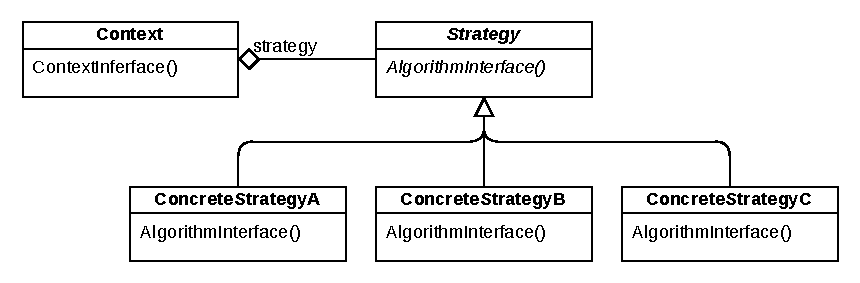
\includegraphics[width=\textwidth]{images/uml_strategy_pattern.pdf}
  \caption{UML class diagram showing the structure of the object-oriented strategy pattern, mimicked in the cpfasst implementation, as defined in \cite{gamma1994design}.}
  \label{fig:uml_strategy_pattern}
\end{figure}

A behavior akin to the object-oriented strategy pattern is implemented as follows, and illustrated in \refFigure{fig:uml_strategy_mimic}:
\begin{figure}[ht]
  \centering
  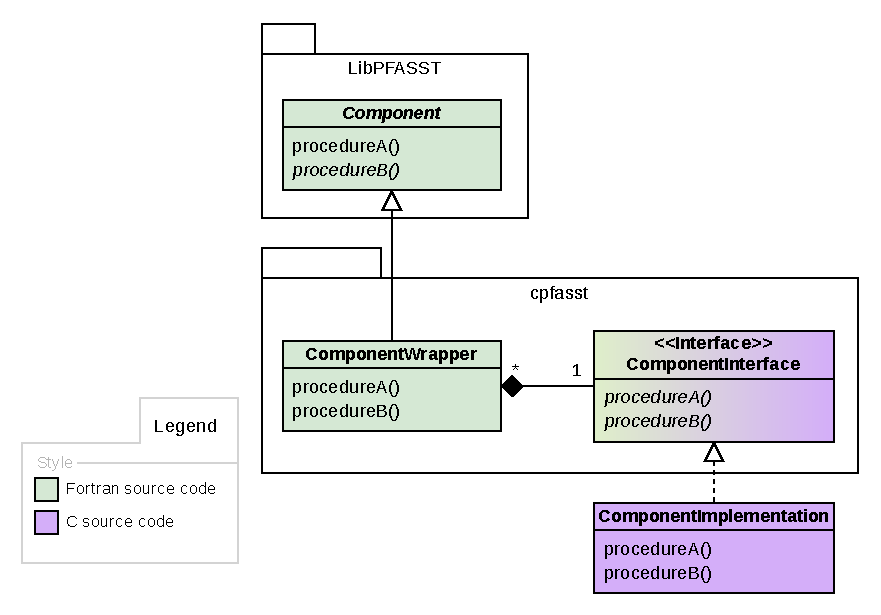
\includegraphics[width=\textwidth]{images/uml_wrapper_pattern.pdf}
  \caption{Pattern used to associate a LibPFASST component with a C implementation, in UML class diagram notation. The LibPFASST abstract component type is extended by a concrete wrapper, which forwards all calls to an interoperable interface, for which the user provides an implementation in C.}
  \label{fig:uml_strategy_mimic}
\end{figure}

\begin{itemize}
    \item For each of the LibPFASST abstract types involved, cpfasst defines, in Fortran, a concrete type extending it --- referred to from now on as a \textit{wrapper type}. The type defines the abstract methods from its parent, and can also override parent methods where needed. It wrapper acts as the pattern's \textit{context}, and all procedures it implements simply forward the call to the \textit{strategy}, performing data type transformations as needed.
    \item The Fortran cpfasst code also declares an interoperable procedure \textit{interface}, with external linkage, corresponding to each of the type's methods. A matching C header file provides equivalent function declarations. Together they act as the abstract \textit{strategy} class.
    \item The cpfasst user imports the header into a source file, and defines each of the contained methods. This implementation acts as the \textit{concrete strategy} class.
\end{itemize}

It's important to note that since the wrapper type delegates the call to specific C functions, this implementation differs from the pattern as used in object-oriented environments, as strategy selection happens at link-time, not runtime. This is a deliberate choice for performance reasons, which will be discussed in \refSection{sec:impl_restrictions}.

For a concrete example of how this pattern is applied, we examine the implementation of the cpfasst interface for the IMEX sweeper, illustrated in \refFigure
{fig:uml_imex_sweeper}. For simplicity, this section assumes the arguments and returns of all procedures to be interoperable, so that they can be passed in calls from Fortran to C without issue.

\begin{figure}[ht]
  \centering
  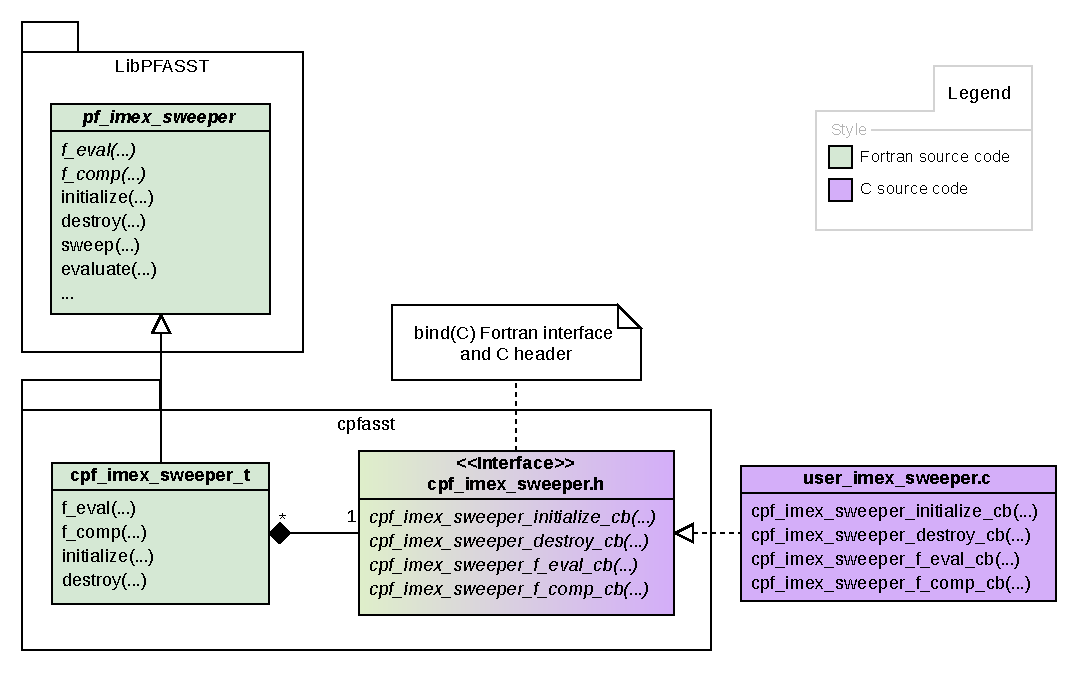
\includegraphics[width=\textwidth]{images/uml_imex_sweeper.pdf}
  \caption{cpfasst implementation of a wrapper type to LibPFASST's IMEX sweeper, in UML class diagram notation.}
  \label{fig:uml_imex_sweeper}
\end{figure}

As mentioned in \refSection{sec:libpfasst_usage}, use of this sweeper in Fortran consists of defining a type extending \ilc{pf_imex_sweeper_t}, and providing implementations
for its deferred type-bound procedures \ilc{f_eval} and \ilc{f_comp}. The cpfasst interface applies the previously described pattern to mimic this usage, implementing the
following elements:
\begin{itemize}
    \item The wrapper Fortran type, \ilc{cpf_imex_sweeper_t}. It provides implementations for \ilc{f_eval} and \ilc{f_comp}, forwarding calls to the corresponding C
    interfaces. Additionally, it also overrides two procedures from the parent type: \ilc{initialize} and \ilc{destroy}. The overriding implementations call both the parent procedure and the corresponding C callback, providing the C implementation an opportunity to initialize and destroy its own private data structures. Note that \ilc{pf_imex_sweeper_t} contains multiple other procedures which are not overridden: as there is no apparent reason why a cpfasst user would need to modify their behavior,
    adding a callback would only clutter the interface.
    \item The interoperable interface is declared twice: once in Fortran, through procedure interfaces with the \ilc{bind(C)} attribute, and once in the C header file 
    \ilc{cpf_imex_sweeper.h}. It is crucial for proper interoperability that the function signatures of both declarations are an exact match, and that types that
    convert between Fortran and C in non-trivial ways, such as character strings, are correctly handled.
\end{itemize}
The C user then imports \ilc{cpf_imex_sweeper.h}, and defines all the functions it declares. The \ilc{f_eval} and \ilc{f_comp} callbacks are an integral part of the solver
and must always be provided, but it is possible that the user implementation has no use for the \ilc{initialize} and \ilc{destroy} callbacks. However, because the
wrapper type calls these interfaces regardless, the C code must still define these functions, even if they are \textit{no-op}s.

\subsection{Data components} \label{sec:impl_data}

With the wrapper types providing referenceable members for all elements of the hierarchy from \refFigure{fig:libpfasst_types}, it is possible to build and run an executable that invokes the C functions at the appropriate contexts. Those functions would be limited to operating on their argument lists, but maintaining the assumption from \refSection{sec:impl_functions} that the argument and return types of all involved procedures are interoperable, this would be sufficient for a simple use case. In fact, LibPFASST's first tutorial, a solution of the 1D Dahlquist test equation, could be replicated in this scenario.

Implementing non-trivial problem-specific behavior under those restrictions, however, is a different matter. When defining a type-bound procedure for one of the extended LibPFASST types in Fortran, the user has full access to the data components from their derived type, and those inherited from the parent type. It follows that cpfasst must provide a mechanism for the C user to achieve similar functionality.

For this, we look again to the object-oriented strategy pattern. As previously mentioned, it provides separation of data between context and strategy --- each of the classes have access to their own member variables, and data is shared between them only through function arguments. When converting from inheritance in a situation where child classes commonly access members variables of the parent class, this can lead to extensive argument lists. Fortunately, this is not the case with LibPFASST. While its code makes little use of accessibility statements for derived type components, and Fortran defaults to public access, its abstract classes are self-contained, with little need for child types to access to parent data --- in fact, it can be argued that LibPFASST components such as the sweeper and user level would be better served by using delegation than inheritance for problem-specific behavior, even Fortran-only code. Where access to parent data is needed, it is restricted to program initialization, by setting parent class variables that control execution behavior. Hence, the same functionality can be covered either by setting those variables during initialization using values provided by a C callback, or by providing get/set interoperable interfaces in Fortran that the C code can call as needed. 

Member data of the strategy class is part the cpfasst user's C code, and as such can be implemented as they see fit --- within some restrictions, which will be discussed in \refSection{sec:impl_restrictions}. It would possible, in fact, to leverage a different object-oriented language's interoperability with C, and implement them as actual members of an object in that language. For C code, the examples provided in with cpfasst illustrate some strategies for implementing data with the desired behavior: for instance, data shared across all objects of a class (equivalent to a C++ static data member) can be represented by a C global variable, in a scope visible to all functions composing the ``class''. This is often the case with problem parameters, such as physical constants or dimensions.

However, there is no easy representation in a purely procedural language for a regular data member (unique to each object). As mentioned in \refSection{sec:impl_functions}, cpfasst is restricted to a single strategy --- a single C ``object'', emulating the functionality of multiple Fortran objects of the same class in LibPFASST. A popular way to emulate this behavior in C --- and, in fact, the way many object-oriented languages, such as C++ and Python, implement class method calls --- is to pass as the first function argument a reference to the ``object'' (a C \ilc{struct} containing the data members). Since in our case the function call comes from Fortran, the Fortran wrapper type must store the reference and pass it as needed: it does so through the interoperable opaque derived type \ilc{c_ptr}. 

\begin{figure}[ht]
  \centering
  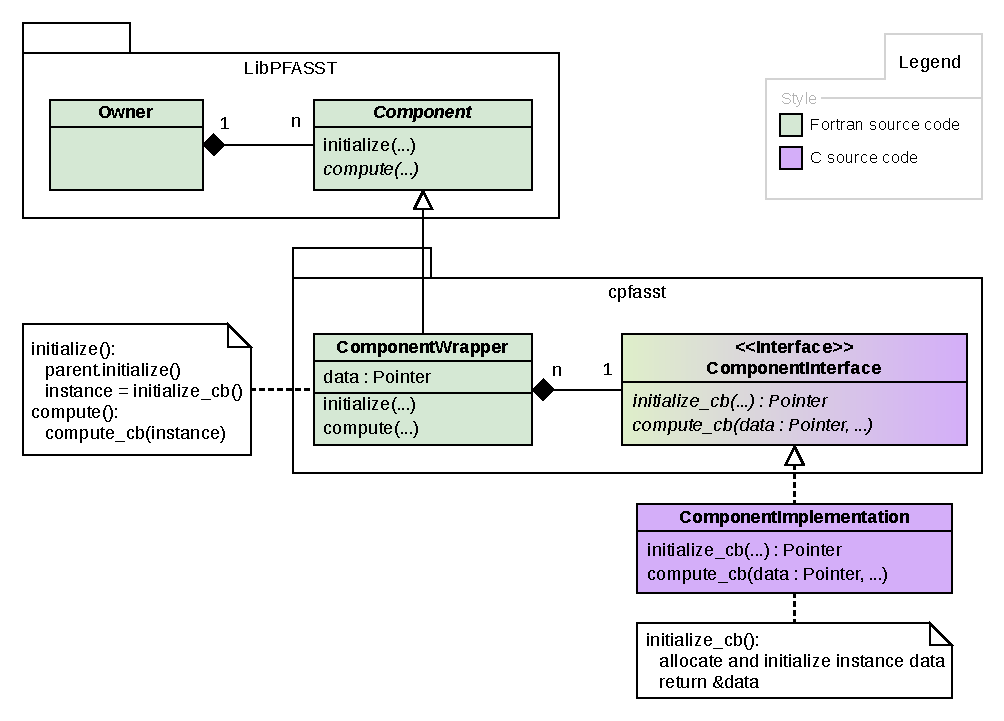
\includegraphics[width=\textwidth]{images/uml_strategy_data.pdf}
  \caption{Pattern used to emulate the behavior of object-oriented data members by the cpfasst interface, in UML class diagram notation. The wrapper type stores a C pointer, which is included as an argument in calls to C callback functions. The data referenced by this pointer is owned by the user's C code, and opaque to the Fortran implementation.}
  \label{fig:uml_strategy_data}
\end{figure}

\refFigure{fig:uml_strategy_data} revisits the diagram from \refFigure{fig:uml_strategy_mimic}, with an emphasis on data members and multiplicities. While the pointer to the user data is stored by the Fortran wrapper type, the data itself is owned by the C code. This includes, if applicable, responsibility for allocating dynamic memory on initialization, and deallocating it on destruction (a callback function not shown in the figure). The wrapper type never changes the pointer's value, and in most cases does not dereference the pointer at all --- the one exception being the wrapper for LibPFASST's data encapsulation type, as detailed in \refSection{sec:impl_functions}.


\subsection{Forwarding non-interoperable procedure calls} \label{sec:impl_calls}

With an understanding of the mechanics cpfasst utilizes for extending Fortran types, we can understand its exact scope. Wrapper types are provided for the abstract types shown in \refFigure{fig:libpfasst_types}: \ilc{pf_encap_t}, \ilc{pf_factory_t} and \ilc{pf_user_level_t} are wrapped directly, but for \ilc{pf_sweeper_t}, only abstract child type \ilc{pf_imex_sweeper_t} is wrapped: interoperable interfaces for other sweepers are outside the scope. Also left outside the scope is \ilc{pf_stepper_t}: it represents a sequential time stepper, and is used only when specified by LibPFASST configuration, for execution of Parareal or for initialization of the coarse level in PFASST --- the respective configuration values are, consequently, not supported. The wrapper functions have the same name as their parents, with the prefix \ilc{pf} replaced by \ilc{cpf}.

In \refSection{sec:impl_oop}, all arguments of type-bound procedures in the wrapper type were assumed to be either of an interoperable type, or easily converted into one. That assumption only holds for a small minority of the procedures the wrapper types must define: most of these procedures take arguments of other derived types. This means we must evaluate interoperability not only for our wrapper types, but also for the types of all arguments in procedures they define (procedures for which a parent definition is inherited are not relevant, as they are not part of the C interface). The results of this analysis are shown in \refFigure{fig:libpfasst_dependencies}.

\begin{figure}[ht]
  \centering
  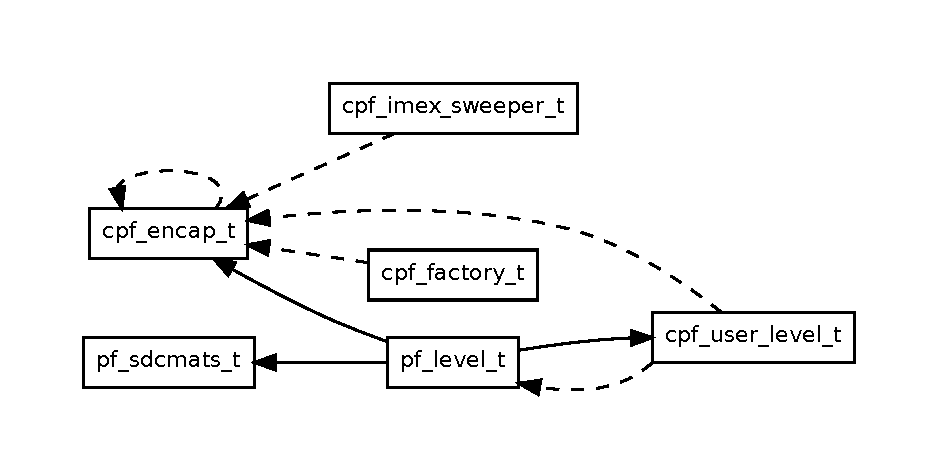
\includegraphics[width=\textwidth]{images/pfasst_dependencies.pdf}
  \caption{Type dependencies of procedures defined by cpfasst wrapper types. A dashed line from A to B indicates that type A contains one or more members of type B. A continuous line from A to B indicates that cpfasst wrapper type A defines a procedure containing an argument of type B (ignoring references to the owner instance).}
  \label{fig:libpfasst_dependencies}
\end{figure}

First, we focus on LibPFASST types appearing in the dependencies: \ilc{pf_level_t} and \ilc{pf_sdcmats_t}. \ilc{pf_stepper_t}, as previously mentioned, is not used within the scope of cpfasst, and can be ignored. Ideally, the remaining types would be interoperable, so that they could be forwarded to the C interfaces without issue: they are not, and cannot easily be converted as they all contain allocatable types. A significant amount of time was spent during development investigating different approaches for interfacing with non-interoperable Fortran types, and the viable strategies created are presented in Appendix \ref{sec:derived_type_interface}. It was ultimately concluded that any maintainable implementation of such an interface for LibPFASST would involve the development of a code generator, and even then might fail to provide the necessary performance for use in the wrapper classes, as all involved procedures are part of the main PFASST execution loop. 

At this point, we approached the issue from a new perspective: how can the non-interoperable types be eliminated from the C interface with minimal restrictions being placed on the cpfasst user? For this, we evaluate each type under the criteria: is there a clear use case where the user needs access to this type? If so, to which components?

\ilc{pf_level_t} appears as an argument in the interpolation and restriction operations, but is not required as an input or output to them: instead, its intended purpose seems to be providing access to the full context of the levels involved. In LibPFASST tutorial and test code, \ilc{pf_level_t} is only used in this context to access user-defined sweeper components for the same level --- this is something the C user's code can easily implement, if needed, based only on that level's index. This allows arguments of \ilc{pf_level_t} to be replaced in the C interface by their respective level indices. Note that access to other members of \ilc{pf_level_t} through the C interface is needed in different contexts, which will be covered separately. \ilc{pf_sdcmats_t}

Having eliminated the dependencies on LibPFASST types, we evaluate the dependencies on the cpfasst wrapper types themselves. While major components of the interoperable interface, they are themselves not interoperable, as they extend other types. This is a considerably easier analysis: a single wrapper type is depended on by all others (including itself), \ilc{cpf_encap_t}. 

\ilc{pf_encap_t} is what is known in other object-oriented languages as a \textit{pure abstract} or \textit{interface} class: it has no data components, and all its type-bound procedures are deferred. As such, when implementing the wrapper \ilc{cpf_encap_t}, there is no need to worry about whether any parent members must be accessible to its procedures, or whether any parent procedures must be overridden to enable extension in C code. Additionally, since the parent has no data components, and according to the mechanisms shown in \refSection{sec:impl_data}, any data components owned by \ilc{cpf_encap_t} are defined in the cpfasst user's C code. Therefore, a dummy argument of type \ilc{cpf_encap_t} can be replaced in the interface by its data pointer.

\section{Initializing LibPFASST components in C} \label{sec:impl_initializing}

In \refSection{sec:impl_oop} we examined how cpfasst allows the user to provide an implementation in C for functionality of LibPFASST types. At this point, it would be possible to run cpfasst code where the solution in space is implemented in C, and LibPFASST initialization and configuration are implemented in Fortran. This might be sufficient for a user comfortable with both languages, but the goal for cpfasst, as mentioned in \refSection{sec:impl_design_goals}, is to support user implementation entirely from C code, hence, we must provide interfaces for initialization and configuration as well. This is approached with a different mindset from the wrapper interfaces: there is no concern for performance, as these steps account for a minimal fraction of the time spent in execution for a real-world application of LibPFASST. Instead, focus is fully shifted into making the interface intuitive and maintainable.

Initialization and configuration in Fortran code involves calls to a few different LibPFASST procedures, as well as allocation and initialization of Fortran user types. Here we run into the same issue described in \refSection{sec:impl_calls}, as the LibPFASST procedures called involve non-interoperable derived types, but in a much more forgiving context. Proper implementation of wrapper types as defined in this work requires that each type-bound procedure call to be forwarded to an equivalent C function, but the procedural nature of initialization and configuration imposes no such constraints: as long as all Fortran steps are executed in a reasonable order, the manner in which they are presented to the C user is of no consequence to LibPFASST operation. In this section, we split this process into three major sections, and examine how each was adapted for the C interface.

\subsection{PFASST configuration} \label{sec:impl_pfasst_config}

This step boils down into correct initialization of the LibPFASST \ilc{pf_pfasst_t} type, which contains variables controlling all LibPFASST configurations, as well as all LibPFASST work variables. In Fortran code, it follows the following sequence:

\begin{enumerate}
    \item \label{config_step_mpi} Initialize MPI by calling \ilc{MPI_Init} \label{config_step_init}
    \item \label{config_step_comm} Initialize the LibPFASST communicator \ilc{pf_comm_t} by calling \ilc{pf_mpi_create} with the appropriate MPI communicator handle
    \item \label{config_step_prm} Initialize the main LibPFASST type \ilc{pf_pfasst_t} by calling \ilc{pf_pfasst_create}, providing the previously initialized \ilc{pf_comm_t}. Optional arguments control how LibPFASST parameters are initialized, which the user can mix as desired. If a value is not provided for a parameter, it is set to a working default (except for \ilc{nlevels}, the number of desired PFASST levels, which is mandatory).
    \begin{itemize}
        \item \ilc{nlevels} can be used to provide a value directly for the mandatory parameter;
        \item \ilc{fname} can be used to provide a path to a file in the Fortran Namelist I/O (nml) format, and the values contained will override LibPFASST defaults;
        \item Unless \ilc{nocmd} provided and set to true, parameters provided in the command line are also read, overriding defaults and those provided by other means.
    \end{itemize}   
\end{enumerate}

Two derived types are involved: \ilc{pf_comm_t} is an internal component of LibPFASST with no contents of interest to the user, so there is no reason to expose it in the C interface. \ilc{pf_pfasst_t}, on the other hand, houses both a set of internal work variables of no interest, and the LibPFASST parameters, which are the key component in this section and must be exposed to the C user. While the internal work variables are non-interoperable, all the parameters are of intrinsic Fortran types, and could easily be converted into interoperable types: taking this into consideration, we evaluated splitting this type into two, with one of the resulting derived types containing only parameters and being interoperable. However, it is unlikely that such a change would be accepted into LibPFASST purely for setup convenience. Even assuming the change was accepted, allowing the interoperable structure containing the parameters to be shadowed in the C interface and directly manipulated by the cpfasst user, the resulting interface might still be unintuitive for use in C code, as it would require character strings to be set according to Fortran convention.

Taking this into consideration, both \ilc{pf_pfasst_t} and \ilc{pf_comm_t} are excluded from the C interface. Step \ref{config_step_mpi} is left to the user's code, allowing MPI to be initialized through the C interface with the desired parameters. Steps \ref{config_step_comm} and \ref{config_step_prm} are condensed in a single interoperable subroutine, \ilc{cpf_initialize}, which takes as arguments the communicator handle obtained from the MPI C interface, and the arguments \ilc{nlevels} and \ilc{fname} from step \ref{config_step_prm}. This subroutine handles the conversion of the MPI handle from C to Fortran (using \ilc{MPI_Comm_f2c}), and the conversion of \ilc{fname} from C string to Fortran string. Argument \ilc{nocmd} is not exposed by the interface, and always set to true in the call to \ilc{pf_pfasst_create} --- testing reveals that the Fortran command line tools are incompatible with a \ilc{main} routine implemented in C, so this feature of LibPFASST cannot be supported.

After the \ilc{cpf_initialize} call, the user can retrieve the resulting parameter values by instantiating the interoperable type \ilc{cpf_parameter_struct}, and initializing it through interoperable subroutine \ilc{cpf_get_parameters}. This copies the relevant parameter values from \ilc{pf_pfasst_t} into a separate interoperable \ilc{struct}, handling string conversions. A corresponding subroutine \ilc{cpf_set_parameters} can be called to copy the values back into \ilc{pf_pfasst_t}, handling string conversions and validating parameter values against any cpfasst restrictions in the process. This is the intended way to initialize parameters for cpfasst, with the nml initialization option being included only as an easy path to reproduce LibPFASST configurations from Fortran for testing.

\subsection{Level configuration}

This step consists of manually instantiating problem-specific components on each of the PFASST levels, as mentioned in \refSection{sec:libpfasst_arch}. The Fortran implementation steps are, for each of the levels:
\begin{enumerate}
    \item Allocate \ilc{pf_user_level_t} using the user-provided concrete type.
    \item Allocate the applicable components of \ilc{pf_user_level_t}: \ilc{pf_factory_t}, \ilc{pf_sweeper_t}, \ilc{pf_stepper_t} using user-provided concrete types or built-in types (where applicable).
    \item \label{config_step_bufsize} Call LibPFASST subroutine \ilc{pf_level_set_size}, providing information about the shape of numeric data used to store the solution for this level.
\end{enumerate}

For cpfasst, the first two steps are straightforward: the wrapper types for each of the LibPFASST types are used, and, as explained in \refSection{sec:impl_calls}, \ilc{pf_stepper_t} is ignored. Step \ref{config_step_bufsize}, however, requires user input: when initializing from Fortran code, the provided shape is used to calculate the size for the MPI buffer used to communicate the level's solution between processors, and on calls to \ilc{pf_factory_t}, where it specifies the desired shape for the data. The latter is only relevant for the built-in factory types (in fact, to avoid confusion regarding row-major/column-major, the corresponding argument is omitted from the C callbacks for \ilc{cpf_factory_t}), but the former is fundamental for correct communication when running with more than one processor.

The \ilc{pf_level_set_size} subroutine takes an optional argument, \ilc{buflen_in}, which allows for directly setting the buffer to the desired length. This is not the storage size, but the required length of a buffer of type \ilc{real(pfdp)} to provide sufficient storage for the solution data. Since the cpfasst solution data is specified in C code by the user and opaque to the Fortran implementation, information about its storage size on each level must be provided by the user in order to correctly configure the MPI buffer.

As before, the steps are condensed into a single interoperable subroutine, \ilc{cpf_initialize_level}, which takes as arguments the level index (zero-based, in accordance with C convention) and the storage size of the solution in bytes. It then allocates all the required wrapper types, converts the solution size to the equivalent buffer length (rounding up if needed) and calls the \ilc{pf_level_set_size}, with a dummy shape of \ilc{[1]} and the calculated buffer length.

\subsection{Running PFASST}

At any point before starting the run, the user must call two cpfasst interoperable subroutines:
\begin{itemize}
    \item \ilc{cpf_set_initial_condition} accepts a reference to an instance of the user-defined solution type, at the finest spatial discretization level,  initialized to the desired initial condition;
    \item \ilc{cpf_set_solution_storage} accepts a separate reference to an instance of the user-defined solution type, at the finest spatial discretization level, which will be used by cpfasst to store the final result of the run.
\end{itemize}
The user retains ownership of this memory, and is responsible for freeing it if dynamically allocated, but must not do so until the run has concluded. The remaining Fortran code steps to start the run are:
\begin{enumerate}
    \item Call LibPFASST subroutine \ilc{pf_pfasst_setup}, which performs final setup steps on the \ilc{pf_pfasst_t}
    \item Call LibPFASST subroutine \ilc{pf_pfasst_run}, providing the desired time step size for the solution, as well as the total number of time steps, which must be a multiple of the number of processors used. This starts PFASST execution.
\end{enumerate}

cpfasst interoperable subroutine \ilc{cpf_run} takes the two arguments described in the second step. It checks that the initial and final condition pointers have been set, then executes the two steps above, starting the run, and returns only when the run is complete. At this point, the user can read the solution from the provided memory. Memory allocated by the Fortran code, or by the user as part of the \ilc{cpf_factory_t} callbacks, should be freed by calling cpfasst subroutine \ilc{cpf_pfasst_destroy}, which calls the LibPFASST procedure of the same name, prompting LibPFASST to free all memory it allocated --- including invoking the \ilc{cpf_factory_t} callbacks to free allocated memory tied to the data encapsulation pointers.


\section{Restrictions of cpfasst functionality} \label{sec:impl_restrictions}

As discussed in \refSection{sec:impl_design_goals}, one of the driving purposes in the development of cpfasst was to expose through the C interface as much of the functionality provided to the Fortran LibPFASST user as possible. However, as mentioned in previous sections, some compromises were imposed by limitations of interoperability, and others by compromises with other design goals. In this section, we detail these limitations and the reasons behind them.

\subsection*{Static linking of callback functions}

As mentioned in Section \refSection{sec:impl_functions}, the cpfasst wrapper types are linked through binding labels to specific C functions. Association of different implementations of user types with different levels can be desirable for purposes such as the use of reduced physics at a coarser level, and is easily achievable for the Fortran user through the creation of different types extending the same LibPFASST abstract type, which are then instanced at the appropriate level. It is possible to implement a wrapper type that behaves in the same manner, by using \ilc{bind(C)} procedures with no binding labels for the callbacks, and the interoperable C function pointer type: the wrapper instance would store C function pointers to each of its callbacks, which would be initialized by the cpfasst user during configuration steps. Aside from the more flexible functionality, the resulting cpfasst interface would arguably be made more intuitive by having the user purposefully provide function pointers to the callbacks, rather than being required to provide definitions for them with specific names.

However, the callback functions are invoked countless times during PFASST execution, and as such, in order to minimize the performance overhead of cpfasst, it is desirable that link-time optimization should be able to apply interprocedural optimizations between the two languages. The GCC 10.1.0 documentation explicitly mentions this feature, but it appears to be limited to direct calls, as testing revealed that functions called through pointers are never inlined. Additionally, link-time warnings about type size mismatches, which are extremely useful for detection of issues in the interoperable interfaces, are not generated for a call made through a function pointer. For this reason, this concept was abandoned in favor of the one presented in this work.

\subsection*{Limited wrapper type callbacks}

When extending abstract types containing non-deferred type-bound procedures, the Fortran user of LibPFASST has the freedom to choose which parent procedures to override, based on problem-specific needs. Due to the static linking of the callback interfaces, however, cpfasst cannot extend this flexibility to the C user: if a wrapper type overrides a parent procedure, forwarding the call to a C callback interface, its definition must be provided by the user in C code. If it does not, the C code has no way to modify that procedure. For some procedures, such as \ilc{initialize} and \ilc{destroy} from \ilc{pf_sweeper_t}, there is a clear use case for overriding them, equivalent to constructor and destructor overriding in other object-oriented languages: just as in those languages, the wrapper type first calls the parent initialization method, then the C callback (corresponding to the child's constructor), with destruction being done in the opposite order. For other procedures, however, even if a callback were provided, should it be invoked before or after the parent procedure? Or replace it entirely? Since there is no clear use case, the inclusion a callback for each parent procedure serves only to increase the complexity of the interface. Thus, we provide callbacks only for deferred type-bound procedures of the parent types, as well as initialize and destroy methods.

\section{Verifying the interoperable interface} \label{sec:impl_verification}

Verification is made significantly harder in multi-language environments. Static code analysis tools and compiler checks are limited to a single language, so while code in each language can be thoroughly checked, the interaction between them remains a potential source of issues. Runtime checks based on code generation in one of the languages are also affected by this, like the checks enabled by gfortran's \ilc{-fcheck=<keyword>} flag. In this section, we highlight tools found during this work to facilitate detection of issues arising from the interaction between languages.

Here it is assumed that all interfaces involved make use of Fortran 2003 C bindings, which, as detailed in \refSection{sec:interop_f03}, preclude multiple issues arising from differences in the low-level representation of a procedure between C and Fortran. Under this assumption, the single major sources of bugs identified is the presence of mismatched representations of an interoperable entity between the two languages.

As explained in \refSection{chapter:interoperability}, every interoperable procedure and type requires a matching representation in Fortran and C. When those representations do not match, it is likely that the code will not operate properly. Unit testing is sufficient to identify more straightforward issues, but others can be extremely hard to diagnose: in the development of cpfasst, a mismatch in the length of a string caused Fortran to read past the bounds of the type it was contained in. This manifested as a segmentation fault, not where the out-of-bounds access occurred, but wherever the next memory allocation was attempted afterwards, and only when running problems above a certain size --- the issue was identified and fixed using the tools discussed here, but the exact reason for how it manifested remains unknown. In \refSection{sec:interop_f90_strings} we discussed a similarly hard to diagnose issue which affected multiple scientific computing tools relying on Fortran 90 interoperability in 2019, the root cause of which was found to be an interface mismatch that had been present for years. It follows that ensuring matching between representations is a critical part of verifying the interface.

\subsection*{Automatically generated headers}

It is possible to automatically generate C headers matching the Fortran representation of interoperable entities using the GNU Fortran compiler's \ilc{-fc-prototypes} flag. In cpfasst, the generated headers were deemed unsuitable for use as the ``official'' interface headers, as prototypes from included modules get placed in a single file, arguments are unnamed, and comments are not carried over. Instead, it was proposed that the generated headers should be included not instead of, but in addition to the manually written ones ---  if the different declarations are not compatible, the compiler stops with a conflicting types error. The downside of using this method is that the error cannot be downgraded into a warning, and sometimes a mismatch in pointer types is deliberate, since the manually written interface includes context that the automatically generated one lacks.

Consider a scenario (for instance, the one described in \refSection{sec:impl_calls}) where the C code passes a pointer to data of arbitrary non-interoperable type to a Fortran procedure, which is then forwarded to a call to a C function: the type of the argument in the Fortran interface declaration is \ilc{type(c_ptr)}, which it translates into the C header as \ilc{void*}. The implementation, however, requires that the referenced data be of a certain type on the first call, and guarantees that it will be of that type on the second --- it makes sense that the pointer type on the manually written header should reflect that. However, when using the generated headers as described above, the mismatch in the pointer type will cause a compilation error, so this trade-off must be considered. The same issue occurs with \ilc{type(c_funptr)}, which generates a pointer of format \ilc{int(*)()}.

\subsection*{Link-time type checks}

One of the best tools for verification of the interoperable interface is easily overlooked, as it is not usually considered a verification tool at all: enabling link-time optimization. When this feature is enabled, the compiler saves its intermediate representation to disk, allowing a single optimization pass at link-time that is not limited to the context of each compiling unit. In GCC, the additional information is also used to perform correctness checks in the types of function arguments: this applies to intrinsic and derived types, passed by reference or value. An example is shown in \refSrc{src:lto_warnings}. In a single-language environment, these additional checks are superfluous, as type mismatches will generate warnings or errors at compile-time. Where the interoperable interface is concerned, however, they are great asset in identifying mismatches between the declaration of the same interface in both languages. Hence, it is strongly recommended that even if link-time optimization is not desirable in a project, it should still be employed for validation.

\begin{listing}
    \inputminted{Fortran}{src/misc/lto_warnings/fsrc.f90}
    \inputminted{C}{src/misc/lto_warnings/csrc.c}
    \inputminted[fontsize=\small]{text}{src/misc/lto_warnings/output.txt}
    \caption{Mismatched declarations of the procedure in C and Fortran cause the code to print incorrect values, but no warnings are generated when linking normally with GCC v10.1.0. With link-time optimization enabled (\ilc{-flto}), type mismatch warnings are issued for both function calls, only one of which is shown here.}
    \label{src:lto_warnings}
\end{listing} 

Since it emits warnings instead of errors, the use of link-time optimization allows the developer to evaluate whether a mismatch is cause for concern and ignore the warning if not. Its main drawbacks are increased compiling and linking time and increased size of the intermediate binaries. Additionally, as mentioned in \refSection{sec:impl_restrictions}, function pointers were found through testing to obfuscate the context of a call to GCC link-time optimization, so calls made through a function pointer are not subject to these checks.

\subsection*{Memory access checks}

Validation of the interface through either of the above methods was found sufficient to ensure equivalence of interoperable entity representations, in the context of the interfaces used for this project. But having correct interface declarations is, as in single-language programs, not sufficient to avoid out-of-bounds memory access in the code using it. Those issues can either arise from the wrapper function code, or from the user's code. The wrapper code is part of the interface, and hence part of the verification process: while Fortran is less prone to out-of-bounds access issues than C, interoperable interfaces often rely on some Fortran intrinsic functions that undermine this robustness by doing the equivalent of a C \textit{cast}, such as \ilc{transfer}, \ilc{c_f_pointer} and \ilc{c_f_procpointer}. Additionally, as previously mentioned, the header generation and link-time check methods are flawed where interoperable Fortran types \ilc{type(c_ptr)} and \ilc{type(c_funptr)} are involved, necessitating the use of additional validation methods to cover those sections.

When it comes to issues in user code, they are not within the scope of interface verification. Nevertheless, it is advisable to offer the user information about verifying their code specifically in the context of interoperable use, as the C/Fortran application seems to be far more sensitive to incorrect memory access than C applications, which are largely unaffected by out-of-bounds reads in memory owned by the program. Furthermore, as mentioned earlier in this section, these issues may not manifest in the manner the C user expects --- of the memory access issues found during development of cpfasst, only a small minority manifested as a segmentation fault tracing back to the instruction where the access occurred --- making information about which tools to use all the more helpful.

Valgrind Memcheck\footnote{\url{https://www.valgrind.org/}} is a well-known tool for dynamic analysis of memory access with MPI support. It instruments a number of instructions related to memory access, detecting accesses to unaddressable memory, memory leaks at program termination, memory aliasing in arguments to functions such as \ilc{strcpy} and \ilc{memcpy}, and use of undefined memory \cite{seward2005using}. Equally relevant in this context is what it does not detect: an access is only considered out-of-bounds by Valgrind when it happens past the boundary of an allocated block on the heap, or on at an invalid address on the stack. An access out-of-bounds in the stack or global memory, for instance, will go undetected so long as it happens in memory the program can legally access. Use of the tool remains recommended, as it would be in a single-language environment, but it was found insufficient for detection of potentially fatal issues in for mixed-language program, and hence should not be solely relied on in such a scenario.

AddressSanitizer\footnote{\url{https://github.com/google/sanitizers/wiki/AddressSanitizer}} is a memory error detector tool, consisting of a compiler instrumentation module and a run-time library. It has been included with GCC since version 4.8, through the \ilc{-fsanitize=address} compiler flag. Its functionality partially overlaps with Valgrind's, but because unlike Valgrind it is able to detect out-of-bounds accesses not only in the heap, but also in the stack and in global memory, as exemplified in \refSrc{src:asan}. It does so by surrounding each variable with ``poisoned'' memory segments, and detecting any access to those segments, both in Fortran and C code. Its main drawback is the need to recompile the code for instrumentation, but at an average memory overhead of 3.4x and runtime increase of 1.73x \cite{serebryany2012addresssanitizer}, it is lightweight enough to be used in development builds for most applications. It is strongly recommended that AddressSanitizer or an equivalent tool be used during verification of interoperable interfaces and user code relying on them.

\begin{listing}
    \inputminted{Fortran}{src/misc/asan/fsrc.f90}
    \inputminted{C}{src/misc/asan/csrc.c}
    \inputminted[fontsize=\small]{text}{src/misc/asan/output.txt}
    \caption{Interoperable code with out-of-bounds memory access in global memory due to mismatched array lengths, and corresponding AddressSanitizer output (edited for brevity). Out-of-bounds accesses in the stack and global variables are not detected by Valgrind Memcheck.}
    \label{src:asan}
\end{listing} 
% !TEX root = ../main.tex
\chapter{Results and analysis}
\label{chapter:results}

\section{The cpfasst interface}

All example code shown in this work, along with suitable build configurations, is hosted in a GitHub repository\footnote{\url{https://github.com/mavma/mlp_examples}}, as is the resulting library code for cpfasst\footnote{\url{https://github.com/mavma/cpfasst}}. Two examples of the use of LibPFASST entirely from C code through the interface are provided by cpfasst. They reproduce the Fortran tutorials of the same name distributed with LibPFASST \cite{libpfasst_ug}:
\begin{itemize}
	\item \textbf{EX2\_Dahlquist} solves the 1D Dahlquist test problem \(y' = \lambda y,\,y(0) = 1\), with an implicit-explicit split \(y' = \lambda_1 y + \lambda_2 y\), where the first term is treated explicitly and the second implicitly, and no grid coarsening in space;
	\item \textbf{EX3\_adv\_diff} solves the 1D linear advection diffusion equation \(u_t = -v u_x + \nu u_{xx}\), with a pseudo-spectral discretization in space and the method of lines in time. In this case, the Fortran tutorial utilizes LibPFASST-provided component \ilc{pf_fft_t}, a fast Fourier transform tool based on fftpack\footnote{\url{https://www.netlib.org/fftpack/}}. Instead of interfacing with the same component, the C example utilizes the C version of fftpack to implement the same functionality: this is intended to demonstrate that code utilizing cpfasst can integrate other C tools as needed.
\end{itemize}

The examples do not only to demonstrate the use of cpfasst, but also are an important part of verification: test scripts are provided to run each of the cpfasst examples and the corresponding LibPFASST tutorial, and compare their outputs. Hence it is important the cpfasst examples reproduce the behavior of their counterparts as faithfully as possible. To support this, the interface code for cpfasst includes not only the major components described in \refChapter{chapter:implementation}, but also get/set interfaces for a handful of additional data components in the main LibPFASST structure.

Each of the LibPFASST tutorials includes a set of nml files containing parameter values for different test cases. These are used in Fortran not only to provide LibPFASST configurations as described in \refSection{sec:impl_pfasst_config}, but also to initialize problem-specific configuration. To facilitate the reproduction of these test cases for the C examples, the interface allows initialization of LibPFASST parameters through nml files, as shown in \refSection{sec:impl_pfasst_config}. Additionally, each C example implements a simplified nml parser, used to read problem-specific parameter values from the LibPFASST-provided configurations --- the user is encouraged to replace this with a C-friendly input format.

Continuous integration runs are set up to compare outputs for each of the examples and tutorials, using each LibPFASST-provided configuration, in sequential and parallel. Output files containing the values of the residual, error and change in initial condition for each sweep executed are compared, and the test is considered successful if the outputs are an exact match. At the LibPFASST output precision of 14 significant digits, all the tests succeed: cpfasst examples match their LibPFASST equivalents exactly. Based on these results, as well as verification of the interface through the methods described in \refSection{sec:impl_verification}, we conclude that cpfasst is suitable for future use in C projects. 

\section{Lessons learned}

The original intent with this development was to quickly implement the C/Fortran interface, and then move on to integration with existing C code or the construction of a Python interface: the expectation was that interfacing with C would be, as described in the LibPFASST's description, \textit{fairly easy}. This is not an unreasonable expectation when it comes to interfacing Fortran and C in general: a good understanding of the Fortran 2003 interoperability features trivializes the creation of C interface for a Fortran library consisting entirely of procedures with sufficiently simple interfaces (no arguments of derived non-interoperable types) which the C user wants to call. Designing the interoperable interface in this case does not require knowledge of how a procedure works, only of what its inputs and outputs should be. Note that a simple interface does not imply trivial library functionality: both LAPACK and BLAS fit this criterion.

LibPFASST, however, presents two major challenges to interoperability:
\begin{enumerate}
	\item \label{problem_oop} \textbf{Object-oriented code} creates an inherent challenge for interfacing with a purely procedural language. This is aggravated by the way LibPFASST use was designed: the user does not use LibPFASST types as much as they provide their own types for LibPFASST to use, which must be created through inheritance, a non-interoperable mechanism.
	\item \label{problem_nested_types} \textbf{Nested non-interoperable types}, which frequently appear as arguments in LibPFASST procedures, cannot be forwarded directly to C calls. Creation of interoperable interfaces for those procedures requires breaking these types down into interoperable components of interest to the user, or omitting them entirely --- which, in turn, requires knowledge of how LibPFASST is implemented and what its potential use cases are.
\end{enumerate}

For both issues, there is no direct solution aside from extensive refactoring of LibPFASST or a change to the Fortran standard --- so instead, we provide paths to work around them. In the case of \ref{problem_oop}, the patterns in Sections \ref{sec:impl_functions} and \ref{sec:impl_data} allow for a sufficiently close approximation of a child class by a combination of cpfasst Fortran code and the user's C code, albeit with some limitations, as discussed in \refSection{sec:impl_restrictions}. When it comes to \ref{problem_nested_types}, no pattern was identified for that can cover all cases: a workaround must be found for each individual procedure depending on its purpose and the types involved. However, the examples discussed in Sections \ref{sec:impl_calls} and \ref{sec:impl_initializing} illustrate successful approaches in different scenarios.

As a consequence of these challenges, design of the C interface became the project itself. Thus, we consider the architecture of the interoperable interface as much a result as the cpfasst code. While cpfasst only provides interfaces for a subset of LibPFASST components, use of the patterns presented in \refSection{sec:impl_oop} and the verification techniques shown in \refSection{sec:impl_verification} will hopefully provide a much smoother path to future work extending the interface to other LibPFASST components.

From the interface design detailed in \refChapter{chapter:implementation}, we synthesize the following guidelines for design of an interoperable interface in Fortran:
\begin{enumerate}
  	\setcounter{enumi}{-1}
	\item \textbf{Use standard interoperability in all interfaces.} Every Fortran procedure called from C, and Fortran interface describing a C function \textit{must} include the \ilc{bind(C)} attribute. As a consequence, the types of all arguments and returns of these procedures must either a \ilc{kind} parameter from the \ilc{iso_c_binding} module, or, for derived types, contain the \ilc{bind(C)} attribute, as described in \refSection{sec:interop_f03}. It can be tempting to ignore this when a non-interoperable component prevents the use of \ilc{bind(C)} and the interface appears to function correctly without it --- however, such an interface relies on compiler-specific or undefined behavior, and can hide a number of issues, detailed in \refSection{sec:interop_f90}. If the compiler disallows (or warns about) usage of a type with \ilc{bind(C)}, it must either be replaced by an equivalent interoperable type, or omitted from the interoperable interface entirely.
	\item \textbf{Employ data encapsulation between languages.} Just as in object-oriented code, allowing access to all data from all contexts may be convenient, but in practice creates an unintuitive and hard to verify interface. It can be useful to see different languages as different object-oriented classes, with a shared understanding of some (interoperable) types, but not others: interoperable types with different conventions in each language (see \refSection{sec:interop_f03}), such as multidimensional arrays (row-major vs column-major) and strings (null-terminated vs blank padded) can be accessed in a manner that is correct when it comes to the underlying data type, but incorrect when it comes to how it is interpreted. Sharing data between languages is best done, as between object-oriented classes, through procedure arguments clearly identified as inputs and outputs, and get/set interfaces which convert between the appropriate conventions as needed. In the specific case of numerical applications, the memory and performance overhead associated with repeated conversion of large multidimensional arrays between row-major and column-major can make this approach non-viable --- in this case, if possible, access to array data should be restricted to a single language, with the other using opaque references if needed: this the approach used by cpfasst, as detailed in Sections \ref{sec:impl_data} and \ref{sec:impl_calls}.
	\item \textbf{Test for interoperability-specific issues during verification.} \refSection{sec:impl_verification} details two types of issues that are of particular interest to an interoperable application: mismatched representation of entities between languages, and out-of-bounds memory accesses in stack and global memory, and discusses tools that can be used to identify them. Here we recommend, in particular, the use of GCC's AddressSanitizer (\ilc{-fsanitize=address}) and link-time optimization features (\ilc{-flto}). Additionally, it is important to adjust expectations about the potential causes of some errors when compared to single-language environments: as a bug in the interface or its use can violate the compiler's assumptions about the application environment, we found that attempting to diagnose an issue such as a segmentation fault with the same approach used for a C-only application will often attribute it to an entirely unrelated area of code, as mentioned in \refSection{sec:impl_verification}.	
\end{enumerate}

Additionally, we recommend the following to designers of new Fortran libraries intended for interoperable use:
\begin{enumerate}
	\item \textbf{Design interfaces that are procedural and interoperable.} All external interfaces should be (non type-bound) procedure calls with the \ilc{bind(C)} attribute. Note that this restricts the use of object-oriented features in the arguments and returns, not in the implementation itself. If it is desirable to offer object-oriented interfaces to Fortran users, this should be done through reuse of the procedural interoperable interfaces --- it is far easier to create object-oriented wrappers for procedural calls than the other way around.
	\item \textbf{If interfaces must be object-oriented, employ delegation.} If association of C function calls with deferred type-bound procedures cannot be avoided, the patterns shown in \refSection{sec:impl_oop} can be employed to build a callback interface. This is greatly facilitated by creation of a type containing only these type-bound procedures (also known in other object-oriented languages as a \textit{pure abstract} or \textit{interface} class). This type can then be used by Fortran code through \textit{delegation}. Additionally, the type-bound procedures should have interoperable argument and return types (excluding the first argument, a reference to the owner object, which in this scenario can never be interoperable). This avoids any concerns about access to parent data (see \refSection{sec:impl_data}), which procedures from the parent type to override (see \refSection{sec:impl_restrictions}) and forwarding non-interoperable arguments (see \refSection{sec:impl_calls}).
\end{enumerate}
% !TEX root = ../main.tex
\chapter{Summary and outlook}
\label{chapter:conclusion}

While the interoperability features introduced by modern Fortran standards greatly facilitate the design of reliable and portable interoperable interfaces, the object-oriented features simultaneously complicate it. While Fortran 90 code could present interoperability challenges even for simple procedure calls, those are precluded by strict adherence to the use of interoperable interfaces as defined in the Fortran 2003 standard. In modern Fortran, we identify as the major obstacle to interoperability the presence of external interfaces relying on non-interoperable features such as object-orientation.

In this project, an interoperable interface was designed for use of select components of the Fortran object-oriented library LibPFASST in C. The resulting library, cpfasst, allows leverage by C code of the parallelization in time features of the PFASST method, creating an opportunity for integration with PDE solvers implemented in C, as well as reuse of the interface by other programming languages that also interoperate with C, such as Python and C++.

As part of development, a design pattern was created for an interoperable interface that exposes functionality equivalent to Fortran type inheritance to the C user. While requiring significant knowledge of the library by the interface designer, and sacrificing some of the flexibility afforded to the Fortran user, the proposed pattern is successful in achieving a flexible user implementation from C. It provides a blueprint for future extension of the interoperable interfaces into different LibPFASST components, as well as for creation of interoperable interfaces for object-oriented Fortran code in general. A set of guidelines relating to design of interoperable interfaces and design of Fortran code intended for interoperability is proposed, deriving from lessons learned during the development of cpfasst.

Proposals for future work in this subject are:
\begin{itemize}
	\item Application of the methods described in this work to expose other components of the LibPFASST to the C user, in particular sweeper types other than implicit-explicit;
	\item Refactoring of LibPFASST code according to the findings presented to allow a more natural interoperable interface;
	\item Study of the performance overhead of the interface in real applications, in particular where it comes to the impact of link-time optimization;
	\item Investigation of the mechanisms behind the manifestation of invalid memory access in stack and global memory as segmentation faults in future attempts at memory allocation.
\end{itemize}

\cleardoublepage
\phantomsection
\addcontentsline{toc}{chapter}{Bibliography}
\bibliography{bibliography/literature}

\part*{Appendix}
\addcontentsline{toc}{part}{Appendix}
\appendix
% !TEX root = ../main.tex
\chapter{Interfaces for non-interoperable derived types} \label{appendix} \label{sec:derived_type_interface}

Once it is determined that a Fortran type appearing as a dummy argument in a procedure call we wish to forward to C code cannot be made interoperable, two approaches were identified in this work to allow the C implementation to access its components. These were ultimately not employed in this work, as the final interface was able to elliminate the non-interoperable arguments entirely, but are presented for didactic purposes with a code example:
\begin{enumerate}
    \item Break the Fortran type down into interoperable components, and pass them as individual arguments to the C function. This is sufficient if the impediment for interoperability of the type is, for instance, an allocatable member of interoperable type. It cannot be used to access deferred-shape array members of derived noninteroperable types, as the argument list would be of unknown size. Its main drawbacks are that it leads to arbitrarily large argument lists, making the C interface hard to read and document, and is hard to code and maintain, with any changes to type structure requiring one (or several, for nested types) arguments to change.
    \item Remove the Fortran type from the argument list, and instead provide a handle as an argument, along with an extensive interface of interoperable getter/setter procedures for individual type components, which the C code can invoke with the handle to manipulate a type\footnote{The getter/setter approach was based on Protocol Buffers (\url{https://developers.google.com/protocol-buffers}), which can be used for interoperability of derived types, providing automated code generation in multiple languages (but not Fortran)}. This approach does not increase complexity of the argument list, and can provide access allocated nested types. It is, however, better suited to automatic code generation than manual coding, as the numerous generated getters and setters would need validation and maintenance, and has the potential to strongly affect performance if invoked from the wrapper callbacks.
\end{enumerate}

\begin{code}
	\inputminted[fontsize=\footnotesize]{Fortran}{src/snippets/derived_type_access.f90}	
\end{code}

\end{document}
